\documentclass[format=acmsmall, review=false, screen=true]{acmart}

\usepackage[utf8]{inputenc}
\usepackage[english]{babel} % typographical and hyphenation rules
\usepackage{amsmath, amsthm, amsfonts}  % loads AMS packages
\usepackage{amssymb}  % provides support for some characters
\usepackage{hyperref} % provides automatic reference types and hyperlinks
\usepackage[noabbrev,capitalize]{cleveref}  % provides automatic reference types
\usepackage{tikz}
\usepackage{mathtools}  % extends amsmath; used in definition of \diag; remove?
\usepackage{thmtools} % used for restating theorems
\usepackage{thm-restate}  % used for restating theorems
\usepackage{emptypage} % used for skipping numbering empty pages
\usepackage{graphicx}
\usepackage{ifthen}

\DeclarePairedDelimiter{\diagfences}{(}{)}
\newcommand{\diag}{\operatorname{diag}\diagfences}

\newcommand{\cL}{{\mathcal{L}}}
\newcommand{\cA}{{\mathcal{A}}}
\newcommand{\defemph}[1]{\textbf{\textsl{#1}}}  % needed?

\newcommand{\Reals}{\mathbb{R}}
\newcommand{\Complex}{\mathbb{C}}
\newcommand{\Rationals}{\mathbb{Q}}
\newcommand{\Algebraics}{\overline{\Rationals}}
\newcommand{\Integers}{\mathbb{Z}}
\newcommand{\Naturals}{\mathbb{N}}

\newcommand{\myvector}{\boldsymbol}

\newcommand{\PTIME}{\textbf{PTIME}}
\newcommand{\NP}{\textbf{NP}}
\newcommand{\coNP}{co-\NP}
\newcommand{\PSPACE}{\textbf{PSPACE}}
\newcommand{\EXPSPACE}{\textbf{EXPSPACE}}

\newcommand{\dist}{\operatorname{dist}}
\DeclarePairedDelimiter{\closurefences}{(}{)}
\newcommand{\closure}{\operatorname{Cl}\closurefences}

\begin{CCSXML}
<ccs2012>
<concept>
<concept_id>10003752.10003753.10003765</concept_id>
<concept_desc>Theory of computation~Timed and hybrid models</concept_desc>
<concept_significance>500</concept_significance>
</concept>
</ccs2012>
\end{CCSXML}

\ccsdesc[500]{Theory of computation~Timed and hybrid models}

\keywords{linear forms in logarithms,
matrix exponential, matrix reachability, matrix logarithms, commuting matrices, hybrid automata}

\acmJournal{JACM}
%\setcopyright{rightsretained}
\setcopyright{acmlicensed}

\title{On the decidability of membership in matrix-exponential semigroups}

\author{Jo\"{e}l Ouaknine}
\authornote{Supported by ERC grant AVS-ISS (648701), and by the Deutsche
Forschungsgemeinschaft (DFG, German Research Foundation) --- Projektnummer 389792660 ---
TRR 248.}
\email{joel@mpi-sws.org}
\author{Amaury Pouly}
\email{pamaury@mpi-sws.org}
\affiliation{
    \institution{Max Planck Institute for Software Systems}
}

\author{Jo\~{a}o Sousa-Pinto}
\orcid{0000-0003-2469-2809}
\email{jspinto@cs.ox.ac.uk}
\author{James Worrell}
\authornote{Supported by EPSRC Fellowship EP/N008197/1}
\email{jbw@cs.ox.ac.uk}
\affiliation{
    \institution{University of Oxford}
}

\begin{abstract}
We consider the decidability of the membership problem for
matrix-exponential semigroups: given $k\in\mathbb{N}$ and square
matrices $A_{1}, \ldots, A_{k}, C$, all of the same dimension and with
real algebraic entries, decide whether $C$ is contained in the
semigroup generated by the matrix exponentials $\exp(A_{i} t)$, where
$i\in\{1,\ldots,k\}$ and $t \geq 0$.  This problem can be seen as a
continuous analog of Babai et al.'s and Cai et al.'s problem of
solving multiplicative matrix equations, and has applications to
reachability analysis of linear hybrid automata and switching systems.
Our main results are that the semigroup membership problem is
undecidable in general, but decidable if we assume that $A_{1},
\ldots, A_{k}$ commute.  The decidability proof is by reduction to a
version of integer programming that has transcendental constants.  We give
a decision procedure for the latter using Baker's theorem on linear
forms in logarithms of algebraic numbers, among other tools.  The
undecidability result is shown by reduction from Hilbert's Tenth
Problem.
\end{abstract}

\begin{document}

\maketitle

\section{Introduction}
Reachability problems are a staple of theoretical computer science and
algorithmic verification. In this paper, our motivation stems from
systems with both continuous variables and discrete control modes.
Systems of this type permeate engineering and the physical sciences:
examples include linear hybrid automata, switching systems,
continuous-time Markov chains, and cyber-physical
systems---see~\cite{Alu15,HenzingerSTOC,HenzingerLICS,AsarinMPS12}.

We focus on systems consisting of a finite number of discrete
control modes (or states), having the property that the continuous
variables of interest evolve in each mode according to some linear
differential equation of the form $\dot{\myvector{x}} = A
\myvector{x}$.  Here $\myvector{x}$ is a vector of continuous
variables, and $A$ is a square `rate' matrix of appropriate dimension.
As is well-known, in each mode the closed form solution
$\myvector{x}(t)$ to the differential equation admits a
matrix-exponential representation of the form $\myvector{x}(t) =
\exp(At)\myvector{x}(0)$. Thus if such a system evolves through a
series of $k$ modes, where the $i$-th mode has rate matrix
$A_i$, then the overall effect on the initial configuration
$\myvector{x}(0)$ is determined by multiplying by the matrix $\prod
\limits_{i=1}^{k} \exp(A_{i} t_{i})$, where $t_i\geq 0$ denotes the
amount of time spent in the $i$-th mode for $i=1,\ldots,k$.  A
particularly interesting situation arises when the matrices $A_i$
commute; in such cases the order in which the
modes are visited (or indeed whether they are visited only once or
several times) is immaterial, the only relevant data being the total
time spent in each mode. Natural questions then arise as to what
kinds of linear transformations can thus be achieved by such systems.

The following decision problem captures a fundamental reachability
question in the setting described above.  The \emph{Matrix-Exponential
  Semigroup Membership Problem (MSMP)} asks, given square matrices
$A_{1}, \ldots, A_{k},C$, all of the same dimension and with
real-algebraic entries, whether $C$ is a member of the matrix
semigroup generated by the set of matrices $\exp(A_i t)$ for
$i\in\{1,\ldots,k\}$ and $t\geq 0$.  The main result of this paper
shows decidability of this problem when the matrices $A_{1}, \ldots,
A_{k}$ commute.  We also show that the problem is undecidable in
general.

\subsection{Related Work}
\label{sec:lics_related_work}

In the case of matrix-exponential semigroups with a single generator,
the membership problem was shown to be decidable in~\cite{Hainry08}
and a polynomial-time procedure was subsequently given
in~\cite{ContinuousOrbitIPL}.  Further reachability problems in the
setting of a single generator are considered
in~\cite{ContinuousSkolem}.

There is a rich literature on membership problems for matrix
semigroups, which can be seen as discrete analogs of the
matrix-exponential semigroups studied in this paper.  Given 
square matrices $A_{1}, \ldots, A_{k}, C$, all of the same dimension,
and with algebraic entries, the \emph{Matrix Semigroup Membership
  Problem} consists in deciding whether the matrix $C$ belongs to the
multiplicative semigroup generated by $\lbrace A_{1}, \ldots, A_{k}
\rbrace$.  A related problem is to determine, given the multiplicative
matrix equation $\prod\limits_{i=1}^{k} A_{i}^{n_{i}} = C$, whether
there is a solution $n_{1}, \ldots, n_{k} \in \Naturals$.  Both
these problems have been shown to be undecidable in
general~\cite{Paterson,MEHTP}.  When the matrices $A_{1}, \ldots,
A_{k}$ commute, the two problems are equivalent, and known to be
decidable~\cite{MultiplicativeMatrixEquations}.  Prior
to~\cite{MultiplicativeMatrixEquations}, the case $k=1$ was shown to
be decidable in~\cite{KL86} and the case $k=2$ was first shown to be
decidable in~\cite{ABC}.  The case $k=2$ without commutativity
assumptions was shown to be decidable in~\cite{MEHTP}.
See~\cite{HalavaSurvey} for a relevant survey, and~\cite{CK05} for
some interesting related problems.

\subsection{Structure of the Paper}
\label{sec:structure}
In order to prove decidability of the Matrix-Exponential Semigroup
Membership Problem in case the generating matrices $A_1,\ldots,A_k$
all commute, we successively reformulate the problem until we
eventually arrive at a version of integer programming that has
transcendental constants.  We show how to solve the latter problem
using Baker's theorem on linear forms in logarithms of algebraic
numbers and results in simultaneous Diophantine approximation.

If matrices $A$ and $B$ commute, then so do their exponentials
$\exp(A)$ and $\exp(B)$.  Using this fact it immediately follows that
in the case of commuting matrices $A_1,\ldots,A_k$, the
Matrix-Exponential Semigroup Membership Problem is equivalent to the
following problem:
\begin{definition}
\label{def:MEP} 
 Given square matrices $A_{1}, \ldots, A_{k}$ and $C$, all of the
  same dimension and with real algebraic entries, the
  \emph{Matrix-Exponential Equation Problem (MEP)} consists in
  determining whether there exist real numbers $t_1,\ldots,t_k \geq 0$
  such that $\prod \limits_{i=1}^{k} \exp(A_{i} t_{i}) = C$.
\end{definition}

The Matrix-Exponential Equation Problem corresponds to reachability in
a switching system in which the number of mode switches is fixed
\emph{a priori}.  Using results in linear algebra about commuting
matrices and basic facts about matrix logarithms, the special case of
the Matrix-Exponential Equation Problem for commuting matrices can be
reduced to the following problem concerning systems of
linear-exponential equations:
\begin{definition}
  An instance of the \emph{Linear-Exponential Equation Problem} (LEP)
  consists of a system of linear-exponential equations in nonnegative
  real variables $t_1,\ldots,t_k$:
\begin{equation}
\begin{aligned}
\textstyle  \exp\left(\sum_{i=1}^k \lambda_i^{(j)} t_i \right) & \, = \, c_j \exp (d_j)
\quad (j=1,\ldots,m)\\
A \boldsymbol{t} & \, = \, \boldsymbol{b} \, , \\
\end{aligned}
\label{single_eqn_form}
\end{equation}
where $k,m\in\mathbb{N}$ and the constants $\lambda_i^{(j)}$, $c_j$,
$d_j$ and the entries of the matrix $A$ and vector $\boldsymbol{b}$
are (possibly complex) algebraic numbers.  The problem asks to
determine whether there exist nonnegative real numbers
$t_1,\ldots,t_k\geq 0$ that satisfy the system
(\ref{single_eqn_form}).
\label{def:LEP}
\end{definition}

By taking logarithms we can reduce the Linear-Exponential Equation Problem
to a version of integer programming with transcendental constants.
More precisely, we consider real constants that can be written as
\emph{linear forms in logarithms of algebraic numbers}, that is,
numbers of the form $\alpha_0+\sum_{i=1}^m \alpha_i\log(\beta_i)$,
where $\alpha_0,\ldots,\alpha_m$ are algebraic numbers and
$\beta_1,\ldots,\beta_m$ are non-zero algebraic numbers (with both the
$\alpha_i$ and $\beta_i$ being possibly complex) and $\log$ is a fixed
branch of the complex logarithm function.
\begin{definition}
An instance of the \emph{Algebraic-Logarithmic Integer Programming
  Problem} (ALIP) consists of a finite system of inequalities of the form
$\pi \Lambda \myvector{x} \leq \myvector{e}$,
where $\Lambda$ is a matrix with real algebraic entries and
where the coordinates of $\myvector{e}$ are real linear forms in
logarithms of algebraic numbers. The problem asks to determine whether
such a system admits a solution $\myvector{x}$ in integers.
\end{definition}

Our strategy to decide the Matrix-Exponential Semigroup
Membership Problem in the commutative case is to establish the
following chain of reductions
\begin{equation*}
\mbox{MSMP} \equiv \mbox{MEP} \leq \mbox{LEP} \leq \mbox{ALIP} 
\end{equation*}
and finally to show decidability of ALIP using results in transcendence
theory and Diophantine approximation.

In the general setting (i.e., without assuming commutativity) we show
that both the Matrix-Exponential Semigroup Membership Problem and the
Matrix-Exponential Equation Problem are undecidable.  The proof is by
reduction from Hilbert's Tenth Problem.  We also show undecidability
of variants of these problems that involve vector reachability and
hyperplane reachability.

\begin{restatable}{definition}{generalisedproblems}
\label{def:generalised-problems}
Given square matrices $A_{1}, \ldots, A_{k}$ and vectors
$\myvector{x}, \myvector{y}$, all of the same dimension and with real
algebraic entries, the \emph{Matrix-Exponential Vector Reachability
  Problem} (MVRP) consists in deciding whether there exists a matrix
$C$ in the semigroup generated by the set
$\lbrace \exp(A_{i} t ): t \geq 0, i = 1,
\ldots, k \rbrace$ such that $C\myvector{x} = \myvector{y}$. 
The \emph{Matrix-Exponential Hyperplane Reachability Problem} (MHRP)
asks whether there exists such a matrix $C$ satisfying
$\myvector{x}^{T} C \myvector{y} = 0$.
\end{restatable}

Our undecidability results will be established by the following chain
of reductions (where HTP refers to Hilbert's Tenth Problem):
\begin{equation*}
\mbox{HTP} \leq \mbox{MEP} \leq \mbox{MSMP} \leq \mbox{MVRP} \leq \mbox{MHRP} \, .
\end{equation*}

\section{Mathematical Background}
\label{ch:background}
In this section we review some results in linear algebra, 
convex geometry, and number
theory.  We also introduce some specialised mathematical
notation that will be needed in the subsequent development.

\subsection{Linear Algebra}

\subsubsection{Jordan Canonical Forms}
\label{sec:jordan}

Let $A \in \Rationals^{d \times d}$ be a square matrix with rational
entries.
The \emph{minimal polynomial} of $A$ is the unique monic
polynomial $m(x) \in \Rationals[x]$ of least degree such that
$m(A)=0$.  By the Cayley-Hamilton Theorem, the degree of $m$ is at most
the dimension of $A$. The set $\sigma(A)$ of eigenvalues is the set of
zeros of $m$, also known as the \emph{spectrum} of $A$.
The \emph{index} of an eigenvalue $\lambda$, denoted
by $\nu(\lambda)$, is its multiplicity as a zero of $m$. We
use $\nu(A)$ to denote $\max_{\lambda\in\sigma(A)} \nu(\lambda)$: the
maximum index over all eigenvalues of $A$. An eigenvalue $\lambda$ is said to be \emph{simple} if $\nu(\lambda) = 1$ and \emph{repeated} otherwise.
Given an eigenvalue $\lambda \in \sigma(A)$, we say that $\myvector{v} \in \Complex^{d}$ is a \emph{generalised eigenvector} of $A$ if $\myvector{v}\in \ker{(A-\lambda I)}^{m}$, for some $m\in\Naturals$.

For each eigenvalue $\lambda$ of $A$, we denote the subspace of
$\Complex^{d}$ spanned by the set of generalised eigenvectors
associated with $\lambda$ by $\mathcal{V}_{\lambda}$. We denote the
subspace of $\Complex^{d}$ spanned by the set of generalised
eigenvectors associated with some real eigenvalue by
$\mathcal{V}^{r}$.  We likewise denote the subspace of $\Complex^{d}$
spanned by the set of generalised eigenvectors associated with some
non-real eigenvalue by $\mathcal{V}^{c}$.

Based on the Jordan decomposition of $A$, as described later on in this 
subsection, each vector $\myvector{v}\in\Complex^{d}$
can be written uniquely as
\begin{equation}
\label{eq:eigen-decomposition}
\myvector{v}=\displaystyle{
  \sum\limits_{\lambda\in\sigma(A)}\myvector{v}_{\lambda}},
\end{equation}
where $\myvector{v}_{\lambda}\in\mathcal{V}_{\lambda}$.
It follows that $\myvector{v}$ can also be uniquely written as
$\myvector{v}=\myvector{v}^{r}+\myvector{v}^{c}$, where
$\myvector{v}^{r} \in\mathcal{V}^{r}$ and
$\myvector{v}^{c} \in\mathcal{V}^{c}$.

We will need the following result:
\begin{proposition}
\label{conj-relation}
  Suppose that $\myvector{v}\in\mathbb{R}^{d}$ and that $\myvector{v}=\sum\limits_{\lambda\in\sigma(A)} \myvector{v}_{\lambda}$, where $\myvector{v}_{\lambda} \in\mathcal{V}_{\lambda}$. For all $\lambda \in \sigma(A)$, it holds that $\myvector{v}_{\overline{\lambda}}$ and $\myvector{v}_{\lambda}$ are component-wise complex conjugates.
\end{proposition}

\begin{proof}
Since $A$ is real, $\myvector{v}_{\lambda}\in \ker{(A-\lambda I)}^{m}$
  implies that
  $\overline{\myvector{v}_{\lambda}} \in \ker{(A-\overline{\lambda}
  I)}^{m}$
  and hence that
  $\overline{ \myvector{v}_{ \overline{\lambda}}} \in
\ker{(A-\lambda I)}^{m}$.  In other words, both $\myvector{v}_{\lambda}$ and
$\overline{ \myvector{v}_{ \overline{\lambda}}}$ lie in
$\mathcal{V}_{\lambda}$.  The result now follows from the fact that
\begin{align*}
\myvector{0}=\myvector{v}-\overline{\myvector{v}}=\sum\limits_{\lambda\in \sigma(A)}(\myvector{v}_{\lambda}-\overline{ \myvector{v}_{ \overline{\lambda}}})
\end{align*}
and from uniqueness of the
decomposition~\eqref{eq:eigen-decomposition}.
\end{proof}

We can write any matrix $A \in \Complex^{d \times d}$ as $A=Q^{-1}JQ$ for some
invertible matrix $Q$ and block diagonal Jordan matrix
$J=\diag{J_{1},\ldots,J_{N}}$, with each block $J_{i}$ having the
following form:

\begin{equation*}
\begin{pmatrix}
\lambda	&&	1		&&	0		&&	\cdots	&&	0		\\
0		&&	\lambda	&&	1		&&	\cdots	&&	0		\\
\vdots	&&	\vdots	&&	\vdots	&&	\ddots	&&	\vdots	\\
0		&&	0		&&	0		&&	\cdots	&&	1		\\
0		&&	0		&&	0		&&	\cdots	&&	\lambda	\\
\end{pmatrix}
\end{equation*}
Moreover, given a rational matrix $A$, its Jordan Normal Form $A=Q^{-1}JQ$ can be
computed in polynomial time, as shown in~\cite{Cai94}.

Note that each vector $\myvector{v}$ appearing as a column of the
matrix $Q^{-1}$ is a generalised eigenvector, and that the
index $\nu(\lambda)$ of each eigenvalue $\lambda$ corresponds to the
dimension of the largest Jordan block associated with it.

One can obtain a closed-form expression for powers of block diagonal
Jordan matrices, and use this to get a closed-form expression for
the powers of a general matrix $A$. In fact, if $J_{i}$ is a
$l\times l$ Jordan block associated with an eigenvalue $\lambda$,
then
%\noindent
\begin{equation}
\label{eq:jordan_powers}
J_{i}^{n}=\begin{pmatrix}
\lambda^{n}	&&	n\lambda^{n-1}	&&	{n\choose 2}\lambda^{n-1}	&&
\cdots		&&	{n\choose l-1}\lambda^{n-l+1}				\\
0			&&	\lambda^{n}		&&	n\lambda^{n-1}				&&
\cdots		&&	{n\choose l-2}\lambda^{n-l+2}				\\
\vdots	&&	\vdots	&&	\vdots	&&	\ddots	&&	\vdots			\\
0		&&	0		&&	0		&&	\cdots	&&	n\lambda^{n-1}	\\
0		&&	0		&&	0		&&	\cdots	&&	\lambda^{n}		\\
\end{pmatrix}
\end{equation}
where ${n\choose j}$ is defined to be $0$ when $n<j$.

\subsubsection{Matrix exponentials}
\label{sec:matrix_exp}

The exponential of a matrix $A \in \Complex^{d \times d}$ is defined
by the power series
\begin{align*}
\exp(A) := \sum \limits_{i=0}^{\infty} \frac{A^{i}}{i!} \in \Complex^{d \times d} \, .
\end{align*}
The series above always converges, and so the exponential of a matrix
is always well defined.  Given $t\in\mathbb{C}$,
one can obtain a closed-form representation of $\exp(At)$ as follows.
Find $Q \in \mathit{GL}_{d}(\Complex)$ such that 
$A=Q^{-1}JQ$ and 
$J=\diag{J_{1},\ldots,J_{N}}$ is a block diagonal Jordan matrix.
Then $\exp(At)=Q^{-1}\exp(Jt)Q$, where $\exp(Jt)=\diag{\exp(J_{1}t),\ldots,\exp(J_{N}t)}$.
Note that due to~\cref{eq:jordan_powers}, if
\begin{align*}
J &= \begin{pmatrix}
\lambda && 1 && 0 && \cdots && 0 \\
0 && \lambda && 1 &&\cdots && 0 \\
\vdots && \vdots && \ddots && \ddots && \vdots \\
0 && 0 && \cdots && \lambda && 1 \\
0 && 0 && \cdots && 0 && \lambda
\end{pmatrix}
\end{align*}
is a Jordan block associated with an eigenvalue $\lambda$, then
\begin{align*}
\exp(Jt) &= \exp(\lambda t) \begin{pmatrix}
1 && t && \frac{t^{2}}{2} && \cdots && \frac{t^{k-1}}{(k-1)!} \\
0 && 1 && t && \cdots && \frac{t^{k-2}}{(k-2)!} \\
\vdots && \vdots &&\ddots && \ddots && \vdots \\
0 && 0 && \cdots && 1 && t \\
0 && 0 && \cdots && 0 && 1
\end{pmatrix} .
\end{align*}

If $A$ and $B$ commute then so do $\exp(A)$ and $\exp(B)$ and in this
case we have $\exp{(A)}\exp{(B)} = \exp{(A+B)}$.

\begin{proposition}
  Let $\myvector{v}$ lie in the generalised eigenspace
  $\mathcal{V}_{\lambda}$ for some $\lambda \in \sigma(A)$.  Then
  $\myvector{b}^{T}\exp(At)\myvector{v}$ is a linear combination
  of terms of the form $t^{n}\exp(\lambda t)$, $n \in \mathbb{N}$.
\label{prop:linear}
\end{proposition}

\begin{proof}
  Note that, if $A=Q^{-1}JQ$ and $J=\diag{J_{1},\ldots,J_{N}}$ is a
block diagonal Jordan matrix, then $\exp(At)=Q^{-1}\exp(Jt)Q$ and
$\exp(Jt)=\diag{\exp(J_{1}t),\ldots,\exp(J_{N}t)}$.  The result
follows by observing that $Q\myvector{v}$ is zero in every component
other than those pertaining the block corresponding to the eigenspace
$\mathcal{V}_{\lambda}$.
\end{proof}

\subsubsection{Matrix Logarithms}
Given a matrix $A \in \Complex^{d \times d}$, define the matrix logarithm
\begin{align*}
\log(A) := \sum \limits_{m=1}^{\infty}(-1)^{m+1} \frac{(A-I)^m}{m} \in \Complex^{d \times d} 
\end{align*}
whenever the above series converges.  In particular the matrix
logarithm is well-defined in case $A$ is unipotent (e.g., when $A$ is
a upper unitriangular matrix) since in this case above series becomes
a polynomial expression in $A$.  In fact it is well-known that the
matrix exponential function and matrix logarithm functions yield a
bijection between nilpotent and unipotent matrices in $\Complex^{d
  \times d}$ (see, e.g.,~\cite[Chapter 2]{Hall15}).  Thus we have:

\begin{proposition}
\label{prop:log_uniqueness}
Given an upper unitriangular matrix $M \in \Complex^{d \times d}$,
there exists a unique strictly upper triangular matrix $L$ such that
$\exp(L)=M$. Moreover, the entries of $L$ lie in the field
$\Rationals(M_{i,j}: 1 \leq i,j \leq d)$ generated over $\mathbb{Q}$
by the entries of $M$.
\end{proposition}

\subsubsection{Properties of commuting matrices}

We present a useful decomposition of $\Complex^{d}$ induced
by the commuting matrices $A_{1}, \ldots, A_{k} \in \Complex^{d \times
  d}$ (cf.~\cite[Section 2]{ABC}). Recall that $\sigma(A_{i})$ denotes
the spectrum of the matrix $A_{i}$ and fix
\begin{align*}
\myvector{\lambda} = (\lambda_{1}, \ldots, \lambda_{k}) \in \sigma(A_{1}) \times \cdots \times \sigma(A_{k}) .
\end{align*}
Note that the generalised eigenspace of $\lambda_{i}$ of $A_{i}$ is equal to $\ker{(A_{i} - \lambda_{i} I)}^{d}$.  (This is because  the increasing sequence ${(\ker{(A_{i} - \lambda_{i} I)}^{n})}_{n \in \Naturals}$ 
of subspaces of $\Complex^d$ must converge in at most $d$ steps.)
With this in mind, we define the following subspace of $\Complex^{d}$:
\begin{align*}
\mathcal{V}_{\myvector{\lambda}} = \bigcap \limits_{i=1}^{k} \ker{(A_{i} - \lambda_{i} I)}^{d}.
\end{align*}
Let $\Sigma = \lbrace \myvector{\lambda} \in \sigma(A_{1}) \times
\cdots \times \sigma(A_{k}) : \mathcal{V}_{\myvector{\lambda}} \neq
\lbrace \myvector{0} \rbrace \rbrace$.  Below, $A_{i}
\restriction_{\mathcal{V}_{\myvector{\lambda}}}$ denotes the
restriction of the linear operator $A_{i}$ to the linear subspace
$\mathcal{V}_{\myvector{\lambda}}$, which is invariant under $A_{i}$.

\begin{theorem}
\label{subspace_decomposition}
For all $\myvector{\lambda} = (\lambda_{1}, \ldots, \lambda_{k}) \in
\Sigma$ and all $i \in \lbrace 1, \ldots, k \rbrace$ the
following properties hold:

\begin{enumerate}

\item $\mathcal{V}_{\myvector{\lambda}}$ is invariant under $A_{i}$.

\item $\sigma(A_{i} \restriction_{\mathcal{V}_{\myvector{\lambda}}}) = \lbrace \lambda_{i} \rbrace$.

\item $\Complex^{d} = \bigoplus \limits_{\myvector{\lambda} \in \Sigma} \mathcal{V}_{\myvector{\lambda}}$.

\end{enumerate}
\end{theorem}

\begin{proof}
We show by induction on $k$ that the subspaces
$\mathcal{V}_{\myvector{\lambda}}$ satisfy the properties above.

When $k = 1$, the result follows from the existence of Jordan Canonical Forms. When $k > 1$, suppose that $\sigma(A_{k}) = \lbrace \mu_{1}, \ldots, \mu_{m} \rbrace$, and let $\mathcal{U}_{j} = \ker{(A_{k} - \mu_{j} I)}^{d}$, for $j \in \lbrace 1, \ldots, m \rbrace$. Again, it follows from the existence of Jordan Canonical Forms that
\begin{align*}
\Complex^{d} = \bigoplus \limits_{j = 1}^{m} \mathcal{U}_{m} .
\end{align*}
Pick $i \in \lbrace 1, \ldots, k-1 \rbrace$ and $j \in \lbrace 1,
\ldots, m \rbrace$. Now, as $A_{k}$ and $A_{i}$ commute, so do
$(A_{k}-\mu_{j} I)$ and $A_{i}$. Therefore, for all $\myvector{v} \in
\mathcal{U}_{j}$, ${(A_{k} - \mu_{j} I)}^{d} A_{i} \myvector{v} =
A_{i} {(A-\mu_{j} I)}^{d} \myvector{v} = \myvector{0}$, so $A_{i}
\myvector{v} \in \mathcal{U}_{j}$, that is, $\mathcal{U}_{j}$ is
invariant under $A_{i}$. The result follows from applying the
induction hypothesis to the commuting operators $A_{i}
\restriction_{\mathcal{U}_{j}}$.
\end{proof}

We will also make use of the following well-known result on simultaneous triangularisation of commuting matrices. See, for example,~\cite{CommutingMatrices}.

\begin{theorem}
\label{thm:simultaneous-triangularisation}
Given commuting matrices $A_{1}, \ldots, A_{k} \in \Complex^{d
  \times d}$, there exists a matrix $P \in \mathit{GL}_{d}(\Complex)$
such that $P^{-1}A_{i}P$ is upper triangular for all $i \in \lbrace 1,
\ldots, k \rbrace$.  Moreover if the entries of every matrix $A_i$ are
algebraic numbers then $P$ may be chosen to have algebraic entries
also.
\end{theorem}

Note that~\cref{thm:simultaneous-triangularisation} will allow us to
reduce general instances of MSMP with commuting matrices to the
subcase where all those matrices are in upper triangular form.

\subsection{Number Theory}

\subsubsection{Linear diophantine equations with algebraic coefficients}
\label{sec:ant}

A complex number $\alpha$ is said to be \emph{algebraic} if it is a
root of some non-zero polynomial with integer coefficients.  The set
of algebraic numbers forms a field, denoted $\Algebraics$. A complex
number that is not algebraic is said to be \emph{transcendental}.

For computational purposes we represent an algebraic number by a
polynomial $P$ with rational coefficients such that $P(\alpha)=0$,
together with a numerical approximation $p+qi$, where
$p,q\in \mathbb{Q}$, of sufficient accuracy to distinguish $\alpha$
from the other roots of $P$~\cite[Section 4.2.1]{Cohen}.  Under this
representation, arithmetic operations and equality testing can be
carried out effectively, as can sign testing of real algebraic numbers

The subfield $\mathbb{K}$ of $\mathbb{C}$ generated by given algebraic
numbers $\alpha_1,\ldots,\alpha_k$ is finite dimensional as a vector
space over $\mathbb{Q}$.  Moreover, given representations of
$\alpha_1,\ldots,\alpha_k$, one can compute a basis of $\mathbb{K}$
over $\mathbb{Q}$ and the (rational) coefficients of each $\alpha_i$
with respect to this basis (see~\cite[Section 4.5]{Cohen}).

\begin{proposition}
    \label{prop:alg_eqn} Let $S=\{ \myvector{x} \in \mathbb{Z}^n :
A\myvector{x}=\myvector{b} \}$, where matrix $A$ and vector
$\myvector{b}$ have algebraic coefficients.  Then we can decide
whether $S$ is non-empty and, if so, can compute
$\myvector{x}_0 \in \mathbb{Z}^d$ and $M \in \mathbb{Z}^{d\times s}$,
for some $s\leq d$, such that $S = \lbrace \myvector{x}_{0} + M \myvector{y}
: \myvector{y} \in \Integers^s \rbrace$.
\end{proposition}

\begin{proof}
Compute a basis $\alpha_1,\ldots,\alpha_k$ of the subfield of
  $\mathbb{C}$ that is generated by the entries of $A$ and
  $\myvector{b}$.  Then we can write $A = \sum_{i=1}^k A_i \alpha_i$
  and $\myvector{b}= \sum_{i=1}^k \myvector{b}_i\alpha_i$, where $A_i$ is a
  matrix of rational numbers of the same dimension as $A$, and
  $\myvector{b}_i$ is a rational vector of the same dimension as
  $\myvector{b}$.  Now we have that
\begin{align*}
A \myvector{x} = \myvector{b} &\Leftrightarrow \left( \sum \limits_{i=1}^{k} A_{i} \alpha_i  \right) \myvector{x} = \sum \limits_{i=1}^{k} \myvector{b}_{i} \alpha_{i} \\
&\Leftrightarrow A_{i} \myvector{x} = \myvector{b}_{i}, \forall i \in \lbrace 1, \ldots, k \rbrace .
\end{align*}

Thus we have characterised $S$ as the set of integer solutions of a
system of equations with rational coefficients.  Now the desired
representation of $S$ can be computed using, e.g., the the procedure
described in~\cite[Chapter X]{Cohen}.
\end{proof}

\subsubsection{Linear Forms in Logarithms}
Let $\log$ denote the principal branch of the complex logarithm
function, i.e., the imaginary part of $\log(z)$ lies in the interval
$(-\pi,\pi]$ for all $z\neq 0$.

Given $k\in\mathbb{N}$, a number $\Lambda$ of the form
\begin{equation}
\Lambda :=  \alpha_{0} + \alpha_{1} \log(\beta_{1}) + \cdots + \alpha_{k} \log(\beta_{k}),
\label{eq:linear-form}
\end{equation}
where $\alpha_{0}, \ldots, \alpha_{n}, \beta_{1}, \ldots, \beta_{k}$
are algebraic numbers, with the $\beta_i$ non-zero, is said to be
a \emph{linear form in logarithms of algebraic numbers}. Note that the
collection of such linear forms is closed under addition, complex
conjugation, and under multiplication by algebraic numbers.

In order to effectively manipulate linear forms we will need 
the following result of Baker~\cite{Baker75}.

\begin{theorem}[Baker]
\label{thm:Baker}
Let $\beta_{1}, \ldots, \beta_{k}$ be non-zero algebraic numbers. If
$\log(\beta_{1}), \ldots, \log(\beta_{k})$ 
are linearly independent over $\Rationals$, then
$1, \log(\beta_{1}), \ldots, \log(\beta_{k})$
are linearly independent over $\Algebraics$.
\end{theorem}

\begin{proposition}
Let $\Lambda = \alpha_0+\sum_{i=1}^k \alpha_i\log(\beta_i) \in \Reals$
be a linear form in logarithms of algebraic numbers for some
nonnegative integer $k$.  Then we can effectively determine the sign
of $\Lambda$ (zero, positive, or negative) and whether
$\frac{\Lambda}{\pi}$ is algebraic.
\label{prop:linear-form-test}
\end{proposition}
\begin{proof}
Clearly we may assume without loss of generality that
$\alpha_1,\ldots,\alpha_k$ are non-zero.  We say that $\Lambda$ is
\emph{reduced} if the set of terms $\mathcal{T}_\Lambda:=\{\log(-1),
\log(\beta_1),\ldots,\log(\beta_k) \}$ is linearly independent over
$\mathbb{Q}$.  Rational linear independence of $\mathcal{T}_\Lambda$
is equivalent to the requirement that the set of multiplicative
relations $\mathcal{L}:=\{ (n_1,\ldots,n_k) \in \mathbb{Z}^k :
\beta_1^{n_1} \cdots \beta_k^{n_k}= 1 \}$ contain only the zero
vector.  Now $\mathcal{L}$ is a subgroup of $\mathbb{Z}^k$ and by a
deep result of Masser~\cite{Mas88} it is possible to compute a basis
of $\mathcal{L}$ (see, e.g.,~\cite{ABC}).  In particular, if $\Lambda$
is not reduced then we can compute an integer linear relation among
$\log(-1),\log(\beta_1),\ldots,\log(\beta_k)$ and rewrite $\Lambda$ so
as to eliminate one of the terms $\log(\beta_i)$ in
$\mathcal{T}_{\Lambda}$.  Continuing in this way we eventually reach an equivalent
reduced form of $\Lambda$.

Suppose that $\Lambda$ is reduced.  Then by Theorem~\ref{thm:Baker}
the set $\{1,\log(-1), \log(\beta_1),\ldots,\log(\beta_k) \}$ is
linearly independent over $\overline{\mathbb{Q}}$.  It follows that
$\Lambda=0$ if and only if $k=0$ and $\alpha_0=0$.  Hence it is
decidable whether or not $\Lambda=0$.  If $\Lambda \neq 0$ then we can
determine the sign of $\Lambda$ by computing a rational approximation
of $\Lambda$ of sufficient precision.  Furthermore we have that
$\Lambda / \pi \in \overline{\mathbb{Q}}$ if and only if $k=1$,
$\alpha_0 = 0$ and $\beta_1 = -1$.
\end{proof}

\subsubsection{Diophantine Approximation}
Given a vector $\myvector{a}\in\Reals^d$ and a set $S\subseteq
\Reals^d$, write $\dist(\myvector{a},S)$ for the $\ell_1$-distance
between $\myvector{a}$ and $S$, i.e., $\inf_{\myvector{b}\in S}
\|\myvector{a}-\myvector{b}\|_1$.  We will need the following
consequence of Kronecker's theorem on simultaneous inhomogeneous
diophantine approximation (see~\cite[Corollary 2.8]{KhachiyanP97}).
\begin{theorem}
\label{thm:kp-density}
Suppose that $\mathcal{C} = \lbrace \myvector{c}_{1}, \ldots, \myvector{c}_{k} \rbrace \subseteq \Reals^{d}$ and that no integer vector is orthogonal to $\mathcal{C}$.
Then for any $\myvector{q} \in \Reals^{d}$
and for any $\varepsilon > 0$ there exist non-negative real numbers $\lambda_{1}, \ldots, \lambda_{k}$ such that
\begin{equation*}
  \dist\left(\myvector{q} + \sum\limits_{i=1}^{k} \lambda_{i} \myvector{c}_{i}, \Integers^{d}\right) \leq \varepsilon \, .
\end{equation*}
\end{theorem}

\subsubsection{Schanuel's Conjecture}
Schanuel's Conjecture~\cite{Lang} is a unifying conjecture in
transcendence theory that generalises many of the classical results in
the field (including~\cref{thm:Baker}).  The conjecture states that if
$\alpha_1,\ldots,\alpha_k \in \mathbb{C}$ are rationally linearly
independent then some $k$-element subset of
$\{\alpha_1,\ldots,\alpha_k,e^{\alpha_1},\ldots,e^{\alpha_k}\}$ is
algebraically independent.

Assuming Schanuel's Conjecture, MacIntyre and Wilkie~\cite{WM} have
shown decidability of the first-order theory of the expansion of the
real field with the exponentiation function and the $\sin$ and $\cos$
functions restricted to bounded intervals.
\begin{theorem}[Wilkie and MacIntyre]
\label{thm:wilkie-macintyre}
  If Schanuel's conjecture is true, then, for each $n \in \Naturals$,
the first-order theory of the strucure $(\Reals,
+, \cdot, \exp, \cos\restriction_{[0, n]}, \sin\restriction_{[0,n]})$
is decidable.
\end{theorem}

\subsection{Convex Geometry}

\subsubsection{Convex Polytopes}

A \emph{convex polytope} is a subset of $\Reals^{n}$ of the form
\begin{equation*}
\mathcal{P} = \lbrace \myvector{x} \in \Reals^{n} : A \myvector{x} \leq \myvector{b} \rbrace ,
\end{equation*}
where $A \in \Reals^{d \times n}$ and $\myvector{b} \in \Reals^{d}$
for some $d\in\mathbb{N}$. When all the entries of $A$ and
$\myvector{b}$ are algebraic numbers, $\mathcal{P}$ is said to have an
algebraic description.  In this case we can decide non-emptiness of
$\mathcal{P}$, e.g., by reduction to the satisfiability problem for the
existential theory of real closed fields.

We will need the following result:
\begin{theorem}[Minkowski-Weyl]
  Any polytope $\mathcal{P} \subseteq \mathbb{R}^{d}$ can be written
  as the sum of two sets $\mathcal{H} \subseteq \mathbb{R}^{d}$ and
  $\mathcal{C} \subseteq \mathbb{R}^{d}$, where $\mathcal{H}$ is a
  finitely generated convex hull and $\mathcal{C}$ is a finitely
  generated cone.
\end{theorem}

\subsubsection{Fourier-Motzkin Elimination}

Fourier-Motzkin elimination is a simple method for eliminating
variables from systems of linear inequalities. The procedure consists
in isolating one variable at a time and comparing all its lower and
upper bounds. Note that this method preserves the set of solutions on
the remaining variables, so a solution of the reduced system can
always be extended to a solution of the original one.

\begin{proposition}
\label{thm:fme}
  It is decidable whether a given convex polytope $\mathcal{P}
  = \lbrace \myvector{x} \in \Reals^{n} : \pi A\myvector{x}
  < \myvector{b} \rbrace$ is empty, where the entries of $A$ are all
  real algebraic numbers and those of $\myvector{b}$ are real linear
  forms in logarithms of algebraic numbers.  Moreover, if
  $\mathcal{P}$ is non-empty then one can compute a rational vector
  $\myvector{q} \in \mathcal{P}$.
\end{proposition}

\begin{proof}
Note that $\mathcal{P}$ is non-empty iff there exists
$\boldsymbol{y} \in \Reals^n$ with $A\myvector {y} < \myvector{b}$.
The existence of such a vector $\boldsymbol{y}$ can be decided using
Fourier-Motzkin elimination.  The linear inequalities that are
generated by the elimination process are such that each coefficient of
a variable $y_i$ is real algebraic and the constant term is a real
linear form in logarithms of algebraic numbers.  Having eliminated all
variables we can decide emptiness since we can effectively decide
whether a real linear form in logarithms is strictly positive by
Proposition~\ref{prop:linear-form-test}.
\end{proof}

\section{Example}
The following example illustrates some elements of our approach to
establishing decidability of the Matrix-Exponential Semigroup
Membership Problem.

Let $\lambda_{1}, \lambda_{2}$ be real algebraic
numbers such that $\lambda_{1} > \lambda_{2}$ and consider the
following commuting matrices $A_{1}, A_{2}$:

\begin{align*}
A_{i} = \begin{pmatrix} \lambda_{i} && 1 \\ 0 && \lambda_{i} \end{pmatrix}, i \in \lbrace 1, 2 \rbrace .
\end{align*}

Given nonnegative real variables $t_{1},t_{2}$ we have that (see Section~\ref{sec:matrix_exp}):
\begin{gather}
\exp(A_{i} t_{i}) = \exp (\lambda_{i} t_{i})
\begin{pmatrix} 1 && t_{i} \\ 0 && 1 \end{pmatrix}, i \in \lbrace 1, 2 \rbrace .
\label{eq:simple-form}
\end{gather}

Let $c_{1}, c_{2}$ be real algebraic numbers such that $c_{1}, c_{2} > 0$, and let
\begin{align*}
C = \begin{pmatrix} c_{1} && c_{2} \\ 0 && c_{1} \end{pmatrix} .
\end{align*}
We would like to determine whether there exist $t_{1}, t_{2} \in \Reals$, $t_{1}, t_{2} \geq 0$ such that
\begin{align}
\exp(A_{1} t_{1}) \exp(A_{2} t_{2}) = C.
\label{eq:goal}
\end{align}

Using the closed-form expression for matrix exponentials
in~(\ref{eq:simple-form}), Equation~(\ref{eq:goal}) is equivalent to
the following pair of equations:
\begin{align*}
\exp(\lambda_{1} t_{1} + \lambda_{2} t_{2}) &= c_{1} \\
(t_{1} + t_{2}) \exp(\lambda_{1} t_{1} + \lambda_{2} t_{2}) &= c_{2} \, .
\end{align*}
Solving directly, we have
\[ t_{1} = \frac{\log(c_{1}) - \frac{c_{2}}{c_{1}} \lambda_{2}}{\lambda_{1} - \lambda_{2}} \quad\text{and}\quad
t_{2} = \frac{\frac{c_{2}}{c_{1}} \lambda_{1} - \log(c_{1})}{\lambda_{1} - \lambda_{2}}
\, . \]
%This amounts to solving the following system of equations:
%\begin{align*}
%&\begin{cases}
%\exp(\lambda_{1} t_{1} + \lambda_{2} t_{2}) = c_{1} \\
%(t_{1} + t_{2}) \exp(\lambda_{1} t_{1} + \lambda_{2} t_{2}) = c_{2}
%\end{cases}
%&\Leftrightarrow \\
%&\begin{cases}
%\exp(t_{1} (\lambda_{1} - \lambda_{2}) + \frac{c_{2}}{c_{1}} \lambda_{2}) = c_{1} \\
%t_{2} = \frac{c_{2}}{c_{1}} - t_{1}
%\end{cases}
%&\Leftrightarrow \\
%&\begin{cases}
%t_{1} = \frac{\log(c_{1}) - \frac{c_{2}}{c_{1}} \lambda_{2}}{\lambda_{1} - \lambda_{2}} \\
%t_{2} = \frac{\frac{c_{2}}{c_{1}} \lambda_{1} - \log(c_{1})}{\lambda_{1} - \lambda_{2}}
%\end{cases}
%\end{align*}

Now  $t_{1}, t_{2} \geq 0$ holds if and only if
\begin{align*}
\lambda_{2} \leq \frac{c_{1}}{c_{2}} \log(c_{1}) \leq \lambda_{1} .
\end{align*}
Whether these inequalities hold amounts to comparing linear forms in
logarithms of algebraic numbers, which is decidable
by~\cref{prop:linear-form-test}.

\section{Decidability in the Commutative Case}
\label{sec:lics_decidability}

We first reduce the Matrix-Exponential Equation Problem (MEP) with
commuting matrices to the Linear-Exponential Problem (LEP), as defined
in Section~\ref{sec:structure}. The idea is to perform a change of
basis so that the matrices $A_{1}, \ldots, A_{k}$, and $C$ in an
instance of MEP all become block-diagonal, with each block being upper
triangular; we then analyse the problem block-wise, making use
of~\cref{prop:log_uniqueness} concerning logarithms of unipotent
matrices.

\begin{proposition}
MEP with commuting matrices reduces to LEP \@.
\label{prop:mep-to-lep}
\end{proposition}

\begin{proof}
  Consider an instance of MEP, as given in \cref{def:MEP},
  with commuting $n\times n$ matrices $A_1,\ldots,A_k$ and target
  matrix $C$.

  We first show how to define a matrix $P$ such that each matrix
  $P^{-1} A_{i} P$ is block diagonal, for $i=1,\ldots,k$, with each block
  being upper triangular.

  By \cref{subspace_decomposition} we can write $\Complex^n$
  as a direct sum of subspaces $\Complex^n = \oplus_{j=1}^m \mathcal{V}_j$
  such that for every subspace $\mathcal{V}_j$ and matrix $A_i$, $\mathcal{V}_j$ is an
  invariant subspace of $A_i$ on which $A_i$ has a single eigenvalue
  $\lambda_i^{(j)}$.

  Define a matrix $Q$ by picking an algebraic basis for each
  $\mathcal{V}_j$ and taking the columns of $Q$ to be the
  successive vectors of each basis.  Then for $i=1,\ldots,k$ the matrix $Q^{-1}
  A_{i} Q$ is block-diagonal, where the $j$-th block is a matrix
  $B^{(j)}_i$ that represents $A_{i} \restriction{\mathcal{V}_j}$,
  $j=1,\ldots,m$.

  Fixing the index of a block $j\in \lbrace 1,\ldots,m \rbrace$, note
  that the matrices $B_1^{(j)},\ldots,B_k^{(j)}$ all commute.  Thus we
  may apply \cref{thm:simultaneous-triangularisation} to obtain an
  algebraic matrix $M_j$ such that each matrix $M_j^{-1} B^{(j)}_{i}
  M_j$ is upper triangular, $i=1,\ldots,k$.  Thus we can write
  \[ M_j^{-1} B^{(j)}_{i} M_j = \lambda_i^{(j)}I + N_i^{(j)} \]
  for some strictly upper triangular matrix $ N_i^{(j)}$.

  We define $M$ to be the block-diagonal matrix
  $M=\mathrm{diag}(M_1,\ldots,M_m)$.  Letting $P=QM$, we have that
  $P^{-1} A_{i} P$ is block-diagonal, with the $j$-th block being
  $\lambda_i^{(j)}I + N_i^{(j)}$ for $j=1,\ldots,m$.  Now for all $t_1,\ldots,t-K\geq 0$ we have
\begin{align}
\prod \limits_{i=1}^{k} \exp \left( A_{i} t_{i} \right) = C \Leftrightarrow \prod \limits_{i=1}^{k} \exp \left( P^{-1}A_{i}P t_{i} \right) = P^{-1}CP .
\label{eq:block}
\end{align}

If $P^{-1}CP$ is not block-diagonal, with each block being upper
triangular and with the same entries along the diagonal, then Equation
(\ref{eq:block}) has no solution and the problem instance must be
negative. Otherwise, denoting the blocks of $P^{-1}CP$ by $D^{(j)}$ for
$j \in \lbrace 1, \ldots, m \rbrace$, our problem amounts to
simultaneously solving the system of matrix equations
\begin{align}
\prod\limits_{i=1}^{k} \exp\left(\left(\lambda_i^{(j)}I + N_i^{(j)}\right)t_{i}\right) = D^{(j)}, \quad j \in \lbrace 1, \ldots, m \rbrace
\label{eq:main1}
\end{align}
where there is one equation for each block.

For each fixed $j$, the matrices $N_{i}^{(j)}$ inherit commutativity from
the matrices $B^{(j)}_{i}$, so we have
\begin{align*}
\prod\limits_{i=1}^{k} \exp \left( (\lambda_i^{(j)}I + N_i^{(j)})t_{i} \right) &=
   \exp \left(\sum_{i=1}^{k} (\lambda_i^{(j)}I  +
 N_i^{(j)}) t_i \right)\\
&= \exp\left(\sum_{i=1}^{k} \lambda_i^{(j)} t_i\right) \cdot
   \exp\left(\sum_{i=1}^{k} N_i^{(j)} t_i \right) .
\end{align*}
Hence the system (\ref{eq:main1}) is equivalent to
\begin{align}
\exp\left(\sum_{i=1}^{k} \lambda_i^{(j)} t_i\right) \cdot
   \exp\left(\sum_{i=1}^{k} N_i^{(j)} t_i \right)  = D^{(j)}
\quad j \in \lbrace 1, \ldots, m\rbrace \, .
\label{eq:main2}
\end{align}

By assumption, the diagonal entries of each matrix $D^{(j)}$ are
all equal to a single value---say $c^{(j)}$.
Since the diagonal entries of
$\exp\left(\sum_{i=1}^{k} N^{(j)}t_i\right)$
are all $1$, the system (\ref{eq:main2}) is equivalent to:
\begin{align*}
\exp\left(\sum_{i=1}^{k} \lambda_i^{(j)} t_i\right)
= c^{(j)} \mbox{ and }\exp\left(\sum_{i=1}^{k} N_i^{(j)} t_i \right)
=\frac{1}{c^{(j)}} D^{(j)}
\end{align*}
for $j=1,\ldots,m$.

Applying~\cref{prop:log_uniqueness}, the
above system can equivalently be written
\begin{align}
\exp\left(\sum_{i=1}^{k} \lambda_i^{(j)} t_i\right)
= c^{(j)} \mbox{ and } \sum_{i=1}^{k}
N_i^{(j)} t_i =
S^{(j)}
\label{eq:almost-final}
\end{align}
for  some effectively computable matrices
$S^{(j)}$ with algebraic entries, $j=1,\ldots,m$.
But the above system of equations is an
instance of LEP\@.
\end{proof}

Next we reduce the Linear-Exponential Equation Problem to the
Algebraic-Logarithmic Integer Programming Problem (ALIP), as defined
in Section~\ref{sec:structure}.

\begin{proposition}
\label{reference-for-log}
LEP reduces to ALIP\@.
\end{proposition}

\begin{proof}
Consider an instance of LEP, comprising a system of equations
\begin{gather}
\textstyle \exp\left(\sum_{\ell=1}^{k} \lambda_\ell^{(j)} t_{\ell} \right) \, = \, c_j \exp (d_j)
\quad j \in \{1,\ldots,m\}, 
\label{eq:LEPinstance}
\end{gather}
and linear equations $A \myvector{t} = \myvector{b}$.

Recall that $\log$ denotes the principal branch of the complex logarithm function.
Note that if any
$c_j=0$ for some $j$ then (\ref{eq:LEPinstance}) has no
solution. Otherwise, by applying $\log$ to each equation in
(\ref{eq:LEPinstance}), we get
\begin{align}
\sum_{\ell=1}^{k} \lambda_\ell^{(j)} t_{\ell} = d_j+\log(c_j) + 2\pi i n_j \quad j\in \{1,\ldots,m\}
\label{eq:logs}
\end{align}
where $n_j \in \Integers$.

The system of equations (\ref{eq:logs}) can be written in matrix form as
\begin{align}
\Lambda \myvector{t} \in \myvector{d}+\log(\myvector{c}) +
2\pi i \Integers^m \, ,
\label{eq:matrixlogs}
\end{align}
where $\Lambda$ is the $m\times k$ matrix with $\Lambda_{j,\ell} = \lambda_\ell^{(j)}$ and $\log$
is applied pointwise to vectors.  A solution to the given instance of LEP comprises
a solution $\myvector{t} \geq 0$ to (\ref{eq:matrixlogs}) that furthermore satisfies 
$A\myvector{t}=\myvector{b}$.  Such a solution exists if and only if the
convex polytope 
\[  \mathcal{T}:=
\lbrace \myvector{x}\in \Reals^m : \exists \myvector{t}\geq
0\, (\myvector{d}+\log(\myvector{c}) + 2\pi i \myvector{x} = \Lambda
\myvector{t} \mbox{ and } A\myvector{t}=\myvector{b}) \rbrace \]
contains an integer point.  

The linear constraints in the definition of $\mathcal{T}$ are such that 
the coefficients of $t_1,\ldots,t_k$ are algebraic and 
the constant terms are linear forms in logarithms of algebraic numbers.
By dividing the equational constraints in the definition of
$\mathcal{T}$ into real and imaginary parts, we can use
Fourier-Motzkin elimination to eliminate the existentially quantified
variables $\myvector{t}$ and arrive at a characterisation
$\mathcal{T}=\{ \myvector{x}: \pi B\myvector{x} \leq \myvector{e}\}$,
for some effectively computable matrix $B$ and vector $\myvector{e}$
such that the entries of $B$ are real algebraic and the entries of
$\myvector{e}$ are real linear forms in logarithms of algebraic
numbers.  But this is the form of an instance of ALIP.
\end{proof}

We are left with the task of showing that ALIP is decidable.  The key
tools here are \cref{thm:kp-density} and \cref{thm:fme}.

\begin{proposition}
ALIP is decidable.
\label{prop:alip}
\end{proposition}

\begin{proof}
We are given a convex polytope $\mathcal{P}=\lbrace \myvector{x} \in
\Reals^{d} : \pi A \myvector{x} \leq \myvector{b} \rbrace$, where the
entries of $A$ are real algebraic and the entries of $\myvector{b}$
are real linear forms in logarithms of algebraic numbers.  We wish to
decide whether $\mathcal{P}$ contains an integer point. 

First we show how to reduce the problem of deciding whether
$\mathcal{P}$ contains an integer point to finitely many instances of
the problem of finding an integer point in a convex polytope $\mathcal{Q}$ of the form
\begin{gather} \mathcal{Q} = \{ \myvector{x}\in \Reals^d : C\myvector{x}=\myvector{d},\,
   \pi E\boldsymbol{x}<\boldsymbol{f} \} \, ,
\label{eq:polyQ}
\end{gather} where the entries of
   $C,E,\boldsymbol{d}$ are real algebraic and the entries of
$\myvector{f}$ are real linear forms in logarithms of algebraic
numbers.  We will obtain a collection of such polytopes $\mathcal{Q}$
from $\mathcal{P}$ by replacing the non-strict inequality ``$\leq$''
in every constraint of $\mathcal{P}$ with either strict inequality
``$<$'' or equality ``$=$''.  To this end, note that when
$\myvector{x} \in \Integers^{d}$, $A \myvector{x}$ is a vector with
algebraic coefficients; so whenever $b_{i} / \pi$ is transcendental
(which can be effectively checked by
Proposition~\ref{prop:linear-form-test}) we may replace the inequality
$\pi(A\boldsymbol{x})_i \leq b_i$ in the definition of $\mathcal{P}$
with a strict inequality $\pi(A\boldsymbol{x})_i < b_i$ without
affecting $\mathcal{P}\cap \Integers^{d}$.  On the other hand,
whenever $b_{i} / \pi$ is algebraic, we split our problem into two
cases: in the first case we replace the inequality
$\pi(A\boldsymbol{x})_i \leq b_i$ with an equality $\pi
(A\boldsymbol{x})_i = b_i$ and in the second case we replace the
inequality $\pi (A\boldsymbol{x})_i \leq b_i$ with the strict
inequality $\pi (A\boldsymbol{x})_i < b_i$.  Thus we obtain a finite
collection of polytopes of the form (\ref{eq:polyQ}).

Next we eliminate the equality constraints in the definition of
$\mathcal{Q}$ so that only strict inequality constraints remain.
Indeed by Proposition~\ref{prop:alg_eqn} we can compute an integer matrix $M$ and
vector $\myvector{x}_0$ such that
\[ \{ \myvector{x} \in \mathbb{Z}^d : C\myvector{x}=\myvector{d} \} =
   \{ \myvector{x}_0 + M\myvector{y} : \myvector{y} \in
   \mathbb{Z}^{d'} \} \] for some $d' < d$.  Then the polytope
   $\mathcal{Q}' := \{ \myvector{y} \in \mathbb{R}^{d'} : \pi
   E(\myvector{x}_0 + M\myvector{y}) < \boldsymbol{f}\}$ contains an
   integer point iff $\mathcal{Q}$ contains an integer point.  Now
   determining the existence of an integer point in a polytope of the
   form $\mathcal{Q}'$ is simply a version of ALIP in which all
   inequality constraints are strict.

It remains to show how to decide whether a polytope $\mathcal{P} :=
\lbrace \myvector{x} \in \Reals^{d}: \pi A \myvector{x} < \myvector{b}
\rbrace$, defined using only strict constraints, contains an integer
point.  To do this we first use Theorem~\ref{thm:fme} to decide
whether $\mathcal{P}$ is non-empty.  In case $\mathcal{P}$ is
non-empty we can use Fourier-Motzkin elimination to find a vector
$\myvector{q} \in \Rationals^{d}$ and $\varepsilon > 0$ such that the
closed $l_1$-ball $\mathcal{B}$ with centre $\myvector{q}$ and radius
$\varepsilon$ with respect to the $l_{1}$ norm is contained in
$\mathcal{P}$.

The next step is to consider the Minkowski-Weyl decomposition of
$\mathcal{P}$, namely $\mathcal{P} = \mathcal{H} + \mathcal{C}$, where
$\mathcal{H}$ is the convex hull of finitely many points of
$\mathcal{P}$ and $\mathcal{C} = \lbrace
\myvector{x} \in \Reals^{d}: A \myvector{x} \leq \myvector{0} \rbrace$
is a cone with an algebraic description.  Note that $\mathcal{P}$ is
bounded if and only if $\mathcal{C} = \lbrace \myvector{0} \rbrace$,
in which case the problem at hand is simple: consider the polytope
$\mathcal{Q}$ with an algebraic description obtained by rounding up
each coordinate of $\myvector{b} / \pi$, which has the same conic part
as $\mathcal{P}$ and which contains $\mathcal{P}$, and therefore is
bounded; finally, compute a bound on $\mathcal{Q}$ (such a bound can
be defined in the first-order theory of the reals), which is also a
bound on $\mathcal{P}$, and test the integer points within that bound
for membership in $\mathcal{P}$. Otherwise,
\begin{align*}
\mathcal{C} = \lbrace \alpha_{1} \myvector{c}_{1} + \cdots + \alpha_{k} \myvector{c}_{k}: \alpha_{1}, \ldots, \alpha_{k} \geq 0 \rbrace,
\end{align*}
where $\myvector{c}_{1}, \ldots, \myvector{c}_{k} \in \Algebraics^{d}$ are the extremal rays of $\mathcal{C}$. Note that $\myvector{q} + \mathcal{C} \subseteq \mathcal{P}$ and that $\mathcal{B} + \mathcal{C} \subseteq \mathcal{P}$.

Now we consider a variation of an argument which appears in~\cite{KhachiyanP97}. Consider the computable set
\begin{align*}
\cL = \mathcal{C}^{\perp} \cap \Integers^{d} \, .
\end{align*}

If $\cL = \lbrace \myvector{0} \rbrace$ then due to~\cref{thm:kp-density} it must be the case that there exist non-negative reals $\lambda_{1}, \ldots, \lambda_{k}$ such that
\begin{align*}
\operatorname{dist} \left(\myvector{q} + \sum\limits_{i=1}^{k} \lambda_{i} \myvector{c}_{i}, \Integers^{d} \right) \leq \varepsilon ,
\end{align*}
and we know that $\mathcal{P} \cap \Integers^{d} \neq \emptyset$ from the fact that the closed ball $\mathcal{B}$ of centre $\myvector{q}$ and radius $\varepsilon$ with respect to the $l_{1}$ norm is contained in $\mathcal{P}$.

On the other hand, if
$\cL \neq \lbrace \myvector{0} \rbrace$, let
$\myvector{z} \in \cL \setminus \lbrace \myvector{0}
\rbrace$.
Since $\mathcal{H}$ is a bounded subset of $\Reals^n$, the set
\[ \lbrace \myvector{z}^T\myvector{x} : \myvector{x}\in \mathcal{P} \rbrace =
   \lbrace \myvector{z}^T\myvector{x} : \myvector{x}\in \mathcal{H} \rbrace \]
is a bounded subset of $\Reals$.
Therefore there exist
$a,b \in \Integers$ such that
\begin{align*}
\forall \myvector{x} \in \mathcal{P}, a \leq \myvector{z}^{T} \myvector{x} \leq b ,
\end{align*}
so we can reduce our problem to $b-a+1$ lower-dimensional instances
by finding the integer points of
$\lbrace \myvector{x} \in \mathcal{P} :
\myvector{z}^{T} \myvector{x} = i \rbrace$,
for $i \in \lbrace a, \ldots, b \rbrace$. Note that we have seen
earlier in the proof how to reduce the dimension of the ambient space
when the polytope $\mathcal{P}$ is contained in an affine
hyperplane.
\end{proof}

Putting together \cref{prop:mep-to-lep}, \cref{reference-for-log}, and \cref{prop:alip}, we obtain:
\begin{theorem}
The Matrix-Exponential Semigroup Membership Problem (as given in \cref{def:MEP}) is decidable in
case the generating matrices $A_1,\ldots,A_k$ commute.
\end{theorem}

\section{Undecidability of the Non-Commutative Case}
\label{sec:lics_encoding}

In this section we show that the Matrix Exponential Equation Problem
and the Matrix-Exponential Semigroup Membership Problem are both
undecidable in general.

\subsection{Matrix-Exponential Equation Problem with Constraints}

The proof of undecidability of  MEP in the non-commutative case is
by reduction from Hilbert's Tenth Problem.  The reduction proceeds via
several intermediate problems.  These problems are obtained by
augmenting MEP with various classes of arithmetic constraints on the
real variables that appear in the statement of the problem.

\begin{definition}
  We consider the following three classes of arithmetic constraints
  over real variables $t_1,t_2,\ldots$:
\begin{itemize}
\item $\mathcal{E}_{\pi\Integers}$ comprises constraints of the form
  $t_{i}\in\alpha+\beta\pi\Integers$, where $\alpha$ and $\beta\neq 0$
  are real-valued constants such that $\cos(2\alpha\beta^{-1})$,
  $\beta$ are both algebraic numbers.
\item $\mathcal{E}_{+}$ comprises linear equations of the form
  $\alpha_1 t_1 + \cdots + \alpha_n t_n = \alpha_0 $, for
  $\alpha_0,\ldots,\alpha_n$ real algebraic constants.
\item $\mathcal{E}_{\times}$ comprises equations of the form
  $t_{\ell} = t_{i} t_{j}$.
\end{itemize}
\end{definition}

These constraints will be useful in defining polynomial relations, as well as in enforcing
that certain variables be integer multiples of $\pi$. They will play a crucial role in the
reduction from Hilbert's Tenth Problem.

A class of constraints $\mathcal{E} \subseteq \mathcal{E}_{\pi\Integers} \cup
\mathcal{E}_{+}\cup \mathcal{E}_{\times}$
induces a generalisation of the MEP problem as follows:
\begin{definition}[MEP with Constraints]
  Given a class of constraints
  $\mathcal{E} \subseteq \mathcal{E}_{\pi\Integers} \cup
  \mathcal{E}_{+}\cup \mathcal{E}_{\times}$,
  the problem MEP$(\mathcal{E})$ is as follows.  An instance consists
  of real algebraic matrices $A_1,\ldots,A_k,C$ and a finite set of
  constraints $E\subseteq\mathcal{E}$ on real variables
  $t_1,\ldots,t_k$.  The question is whether there exist non-negative
  real values for $t_1,\ldots,t_k$ such that
  $\prod_{i=1}^{k} e^{A_{i} t_{i}}=C$ and the constraints $E$ are all
  satisfied.
\label{def:contraintMEP}
\end{definition}

Note that in the above definition of MEP$(\mathcal{E})$ the set of
constraints $E$ only utilises real variables $t_1,\ldots,t_k$
appearing in the matrix equation $\prod_{i=1}^{k} e^{A_{i} t_{i}}=C$.
However, without loss of generality, we can allow constraints to
utilise fresh variables $t_{i}$, for $i>k$, since we can always define a
corresponding matrix $A_i=0$ for such variables for then
$e^{A_{i} t_{i}}=I$ has no effect on the matrix product.  In other words,
we can without loss of generality have constraints in $\mathcal{E}$ with existentially
quantified variables.  In particular, we have the following
useful observations:

\begin{itemize}
\item[\textbullet] We can express inequality constraints of the form
  $t_{i}\neq \alpha$ in  $\mathcal{E}_{+}\cup \mathcal{E}_{\times}$ by
using fresh variables
  $t_{j},t_{\ell}$.  Indeed $t_{i} \neq \alpha$ is satisfied whenever there
  exist values of $t_{j}$ and $t_{\ell}$ such that $t_{i}=t_{j}+\alpha$ and
  $t_{j} t_{\ell}=1$.

\item[\textbullet] By using fresh variables,
  $\mathcal{E}_{+}\cup \mathcal{E}_{\times}$ can express polynomial
  constraints of the form $P(t_1,\ldots,t_n)=t$ for $P$ a polynomial
  with integer coefficients.
\end{itemize}

We illustrate the above two observations in an example.
\begin{example}
  Consider the problem, given matrices $A_1,A_2$ and $C$, to decide
  whether there exist $t_1,t_2 \geq 0$ such that
  \[ e^{A_1t_1}e^{A_2t_2}=C \,\mbox{ and }\, t_1^2-1=t_2, t_2\neq 0 \, .\]
  This is equivalent to the following instance of
  MEP$(\mathcal{E}_{+}\cup\mathcal{E}_{\times})$: decide whether there exist $t_1,\ldots,t_5\geq 0$ such that
\[ \prod_{i=1}^5 e^{A_{i} t_{i}}=C \,\mbox{ and }\, t_1t_1=t_3, t_3-1=t_2, t_2t_4=t_5, t_5=1\]
where $A_1,A_2$ and $C$ are as above and $A_3=A_4=A_5=0$.
\end{example}

We will make heavy use of the following proposition to combine several
instances of the constrained MEP into a single instance by combining
matrices block-wise.
\begin{proposition}\label{prop:remark}
  Given real algebraic matrices $A_1,\ldots,A_k,C$ and
  $A_1',\ldots,A_k',C'$, there exist real algebraic matrices
  $A_1'',\ldots,A_k''$, $C''$ such that for all $t_1,\ldots,t_k$:
  \[\prod_{i=1}^{k} e^{A_{i}''t_{i}}=C''\qquad\Leftrightarrow\qquad\left(\prod_{i=1}^{k} e^{A_{i} t_{i}}=C\right)\wedge\left(\prod_{i=1}^{k} e^{A_i't_{i}}=C'\right).\]
\label{prop:combine}
\end{proposition}

\begin{proof}
For any $i\in \lbrace 1,\ldots,k \rbrace$, define
\[A_i''=\begin{bmatrix}A_i&0\\0&A_i'\end{bmatrix},\qquad
C''=\begin{bmatrix}C&0\\0&C'\end{bmatrix}.\]
The result follows because the matrix exponential can be computed
block-wise (as is clear from its power series definition):
\[\prod_{i=1}^{k} e^{A_i''t_{i}}=\prod_{i=1}^{k}\begin{bmatrix}e^{A_{i} t_{i}}&0\\0&e^{A_i't_{i}}\end{bmatrix}=
\begin{bmatrix}\prod_{i=1}^{k} e^{A_{i} t_{i}}&0\\0&\prod_{i=1}^{k} e^{A_i't_{i}}\end{bmatrix}.\]
\end{proof}

We remark that in the statement of \cref{prop:remark} the
two matrix equations that are combined are over the same set of
variables.  However, we can clearly combine any two matrix equations
for which the common variables appear in the same order in the
respective products.

The core of the reduction is to show that the constraints in
$\mathcal{E}_{\pi\Integers},\mathcal{E}_{+}$ and
$\mathcal{E}_{\times}$ do not make the MEP problem harder.

\begin{proposition}
  MEP$(\mathcal{E}_{\pi\Integers} \cup \mathcal{E}_{+} \cup
  \mathcal{E}_{\times})$ reduces to MEP$(\mathcal{E}_{+} \cup
  \mathcal{E}_{\times})$.
\label{lem:pi}
\end{proposition}
\begin{proof}
  Let $A_1,\ldots,A_k,C$ be real algebraic matrices and
  $E\subseteq \mathcal{E}_{\pi\Integers} \cup \mathcal{E}_{+} \cup
  \mathcal{E}_{\times}$
  a finite set of constraints on real variables $t_1,\ldots,t_k$.  Since $E$ is
  finite it suffices to show how to eliminate a single constraint
  in $\mathcal{E}_{\pi \Integers} \cap E$ from $E$.

  Let $t_{j}\in\alpha+\beta\pi\Integers$ be a constraint in $E$.  By definition
of  $\mathcal{E}_{\pi\Integers}$
we have
  that $\beta \neq 0$ and that both $\beta$ and $\cos(2\alpha\beta^{-1})$
   are real algebraic.  The Pythagorean theorem implies that $\sin(2\alpha\beta^{-1})$ is also real algebraic.  Now define the following extra
  matrices:
\[A'_j=\begin{bmatrix}0&2\beta^{-1}\\-2\beta^{-1}&0\end{bmatrix},
 C'=\begin{bmatrix}\cos(2\alpha\beta^{-1})&
\sin(2\alpha\beta^{-1})\\-\sin(2\alpha\beta^{-1})&\cos(2\alpha\beta^{-1})\end{bmatrix}.\]
Our assumptions ensure that $A_j'$ and $C'$ are both real algebraic.

We now have the following chain of equivalences:
\begin{align*}
e^{A'_j t_{j}}=C'
&\Leftrightarrow\begin{bmatrix}\cos(2t_{j}\beta^{-1})&
\sin(2t_{j}\beta^{-1})\\-\sin(2t_{j}\beta^{-1})&\cos(2t_{j}\beta^{-1})\end{bmatrix}
=C'\\
&\Leftrightarrow\cos(2t_{j}\beta^{-1})=\cos(2\alpha\beta^{-1}) \\
&\qquad\wedge\sin(2t_{j}\beta^{-1})=\sin(2\alpha\beta^{-1}) \\
  &\Leftrightarrow2\beta^{-1}t_{j}\equiv 2\alpha\beta^{-1} \pmod{2\pi} \\
&\Leftrightarrow t_{j}\in\alpha+\beta\pi\Integers.
\end{align*}
Thus the additional matrix equation $e^{A_j't_{j}}=C'$ is equivalent to
the constraint $t_{j}\in\alpha+\beta\pi\Integers$.  Applying
\cref{prop:combine} we can thus eliminate this constraint.
\end{proof}

\begin{proposition}
  MEP$(\mathcal{E}_{+}\cup\mathcal{E}_{\times})$ reduces to
  MEP$(\mathcal{E}_{+})$.
\label{lem:times}
\end{proposition}

\begin{proof}
  Let $A_1,\ldots,A_k,C$ be real algebraic matrices and
  $E \subseteq\mathcal{E}_{+}\cup\mathcal{E}_{\times}$ a finite set of
  constraints on variables $t_1,\ldots,t_k$.  We proceed as above,
  showing how to remove each constraint in
  $\mathcal{E}_{\times}$ from $E$.  In so doing we potentially increase the
  number and the dimension of matrices and add new constraints from $\mathcal{E}_{+}$.

  Let $t_l=t_{i} t_{j}$ be an equation in $E$.  To eliminate this equation
the first step is to introduce fresh
variables $x,x',y,y',z$ and add the constraints
\[ t_{i}=x,\, t_{j}=y,\, t_{\ell} = z,\]
which are all in $\mathcal{E}_{+}$.  We now add a new matrix equation
over the fresh variables $x,x',y,y',z$ that is equivalent to the
constraint $xy=z$.  Since this matrix equation involves a new set of
variables we are free to the set the order of the matrix products,
which is crucial to express the desired constraint.

The key gadget is the following matrix product equation,
  which holds for  any $x,x',y,y',z\geqslant0$:
\begin{equation*}
\begin{bmatrix}1&0&-z\\0&1&0\\0&0&1\end{bmatrix}
\begin{bmatrix}1&0&0\\0&1&-y'\\0&0&1\end{bmatrix}
\begin{bmatrix}1&x&0\\0&1&0\\0&0&1\end{bmatrix}
\begin{bmatrix}1&0&0\\0&1&y\\0&0&1\end{bmatrix}
\begin{bmatrix}1&-x'&0\\0&1&0\\0&0&1\end{bmatrix}=
\begin{bmatrix}1&x-x'&z-xy\\0&1&y-y'\\0&0&1\end{bmatrix}.
\end{equation*}

Notice that each of the matrices on the left-hand side of the above
equation has a single non-zero off-diagonal entry.  Crucially each
matrix of this form can be expressed as an exponential.  Indeed we can
write the above equation as a matrix-exponential product
\[ e^{B_1z} e^{B_2y'} e^{B_3x} e^{B_4y} e^{B_5x'} = \begin{bmatrix}1&x-x'&z-xy\\0&1&y-y'\\0&0&1\end{bmatrix} \]
for matrices
\begin{align*}
&B_1=\begin{bmatrix}0&0&-1\\0&0&0\\0&0&0\end{bmatrix} &&
&B_3=\begin{bmatrix}0&1&0\\0&0&0\\0&0&0\end{bmatrix} &&
B_5=\begin{bmatrix}0&-1&0\\0&0&0\\0&0&0\end{bmatrix} \\[10pt]
&B_2=\begin{bmatrix}0&0&0\\0&0&-1\\0&0&0\end{bmatrix} &&
&B_4=\begin{bmatrix}0&0&0\\0&0&1\\0&0&0\end{bmatrix} \\
\end{align*}
Thus the constraint $xy=z$ can be expressed as
\begin{gather}
e^{B_1z} e^{B_2y'} e^{B_3x} e^{B_4y} e^{B_5x'} = I \, .
\label{eq:fresh}
\end{gather}

Again, we can apply \cref{prop:combine} to combine the
equation (\ref{eq:fresh}) with the matrix equation from the original
problem instance and thus encode the constraint $z=xy$.
\end{proof}

\begin{proposition}
  MEP$(\mathcal{E}_{+})$ reduces to MEP\@.
\label{lem:plus}
\end{proposition}

\begin{proof}
  Let $A_1,\ldots,A_k,C$ be real algebraic matrices and
  $E \subseteq\mathcal{E}_{+}$ a set of constraints.
  We proceed as above, showing how to eliminate each constraint from
  $E$ that lies in $\mathcal{E}_{+}$, while preserving the set of
  solutions of the instance.

Let $\beta+\sum_{i=1}^{k} \alpha_{i} t_{i}=0$ be an equation in $E$.
Recall that $\beta,\alpha_1,\ldots,\alpha_k$ are real algebraic.
Define the extra matrices $A_1',\ldots,A_k'$ and $C'$ as follows:
\[A_i'=
\begin{bmatrix}
  0&\alpha_{i} \\
  0&0
\end{bmatrix},
\qquad C'=\begin{bmatrix}
1&-\beta \\
0&1\end{bmatrix}.
\]
Our assumptions ensure that $A_1',\ldots,A_k'$ and $C'$ are all real algebraic.
Furthermore, the following extra product equation becomes:
\begin{align*}
\prod_{i=1}^{k} e^{A_i't_{i}}=C &\Leftrightarrow
\prod_{i=1}^{k}\begin{bmatrix}
1&\alpha_{i} t_{i} \\
0&1
\end{bmatrix}=\begin{bmatrix}
1&-\beta \\
0&1
\end{bmatrix}\\
&\Leftrightarrow\sum_{i=1}^{k}\alpha_{i} t_{i}=-\beta \, .
\end{align*}
The result follows by applying \cref{prop:combine}.
\end{proof}

Combining~\cref{lem:pi}, \cref{lem:times}, and \cref{lem:plus} we
have:
\begin{proposition}
  MEP$(\mathcal{E}_{\pi\Integers}\cup\mathcal{E}_{+}\cup\mathcal{E}_{\times})$
  reduces to MEP\@.
\end{proposition}

\subsection{Reduction from Hilbert's Tenth Problem}

\begin{theorem}
  MEP is undecidable in the non-commutative case.
\end{theorem}

\begin{proof}
  We have seen in the previous section that the problem
  MEP$(\mathcal{E}_{\pi\Integers}\cup\mathcal{E}_{+}\cup\mathcal{E}_{\times})$
  reduces to MEP without constraints.  Thus it suffices to reduce
  Hilbert's Tenth Problem to
  MEP$(\mathcal{E}_{\pi\Integers}\cup\mathcal{E}_{+}\cup\mathcal{E}_{\times})$.
  In fact the matrix equation will not play a role in the
  target of this reduction, only the additional constraints!

  Let $P$ be a polynomial of total degree $d$ in $k$ variables with
  integer coefficients. From $P$ we build a homogeneous polynomial $Q$, by
  adding a new variable $\lambda$:
  \[Q(\mathbf{x},\lambda)=\lambda^{d}P\left(\frac{x_1}{\lambda},\ldots,
    \frac{x_k}{\lambda}\right).\]
  Note that $Q$ still has integer coefficients. Furthermore, we have the relationship
\[Q(\mathbf{x},1)=P(\mathbf{x}).\]

As we have seen previously, it is easy to encode $Q$ with constraints,
in the sense that we can compute a finite set of constraints
$E_Q \subseteq \mathcal{E}_{+}\cup\mathcal{E}_{\times}$ utilising variables
$t_0,\ldots,t_m,\lambda$
such that $E$ is
satisfied if and only if $t_0=Q(t_1,\ldots,t_k,\lambda)$. Note that
$E_Q$ may need to utilise variables other
than $t_1,\ldots,t_k$ to do that.  Another
finite set of equations
$E_{\pi\Integers}\subseteq\mathcal{E}_{\pi\Integers}$ is used to
encode that $t_1,\ldots,t_k,\lambda\in\pi\Integers$. Finally,
$E_{=}\subseteq\mathcal{E}_{+}\cup\mathcal{E}_{\times}$ is used to
encode $t_{0}=0$ and $1\leqslant \lambda\leqslant4$.  The
latter is done by adding the polynomial equations $\lambda=1+\alpha^2$ and
$\lambda=4-\beta^2$ for some $\alpha$ and $\beta$. Finally we have the
following chain of equivalences:
\begin{align*}
&\exists t_0,\ldots,\lambda\geqslant0\text{ s.t. }E_Q\cup E_{\pi\Integers}\cup E_{=}\text{ is satisfied }\\
&\qquad\Leftrightarrow\exists t_1,\ldots,\lambda\geqslant0\text{ s.t. } 0=Q(t_1,\ldots,t_k,\lambda)\\
    &\qquad\qquad\wedge t_1,\ldots,t_k,\lambda\in\pi\Integers\wedge 1\leqslant\lambda\leqslant4\\
&\qquad\Leftrightarrow\exists n_1,\ldots,n_k\in\Naturals\text{ s.t. } 0=Q(\pi n_1,\ldots,\pi n_k,\pi)\\
&\qquad\Leftrightarrow\exists n_1,\ldots,n_k\in\Naturals\text{ s.t. } 0=\pi^{d} Q(n_1,\ldots,n_k,1)\\
&\qquad\Leftrightarrow\exists n_1,\ldots,n_k\in\Naturals\text{ s.t. } 0=P(n_1,\ldots,n_k).\\
\end{align*}
\end{proof}

\subsection{Enforcing a Matrix Product Order}
\label{sec:lics_gadget}

In this section, we will present a gadget matrix-exponential semigroup that can
enforce a certain partial order on the matrices reaching a particular target.
This will be useful to establish the reduction MEP $\leq$ MSMP\@.
More precisely, we will exhibit five matrices $W,X,Y,Z$ and $G$ such that any
product $G=\prod_{i=1}^{p} e^{A_{i} t_{i}}$
where $t_{i}>0$ and $A_{i}\in \lbrace W,X,Y,Z \rbrace$ is such that all the ``$X$'' appear before
the ``$Y$''. Define the following matrices:

\begin{align*}
W&=\begin{bmatrix}0&0&0\\0&1&0\\0&0&2\end{bmatrix},&&
&X=\begin{bmatrix}0&0&0\\0&0&1\\0&0&0\end{bmatrix},&&
Z=\begin{bmatrix}0&0&0\\0&-1&0\\0&0&-2\end{bmatrix},\\[5pt]
Y&=\begin{bmatrix}0&1&0\\0&0&0\\0&0&0\end{bmatrix},&&
&G=\begin{bmatrix}1&1&0\\0&1&1\\0&0&1\end{bmatrix}.\\
\end{align*}
One easily computes the exponentials $W,X,Y,Z$:
\[
e^{Wt}=\begin{bmatrix}1&0&0\\0&e^t&0\\0&0&e^{2t}\end{bmatrix},
e^{Xt}=\begin{bmatrix}1&0&0\\0&1&t\\0&0&1\end{bmatrix},
e^{Yt}=\begin{bmatrix}1&t&0\\0&1&0\\0&0&1\end{bmatrix},
e^{Zt}=\begin{bmatrix}1&0&0\\0&e^{-t}&0\\0&0&e^{-2t}\end{bmatrix}.
\]

The crux of the proof will be based on the following asymmetry between $X$ and $Y$,
which leaves the top right corner zero in one case but nonzero in the other. As we will later
observe, once the top right corner is nonzero, it cannot be cleared.
\[
e^{Xt}e^{Yu}=\begin{bmatrix}1&u&0\\0&1&t\\0&0&1\end{bmatrix},\qquad
e^{Yt}e^{Xu}=\begin{bmatrix}1&u&tu\\0&1&t\\0&0&1\end{bmatrix}.
\]

\begin{proposition}\label{prop:eq_has_forced_order}
If there exist $p\in\Naturals$, $A_{i}\in\lbrace W,X,Y,Z\rbrace$ and $t_{i}>0$, for $i\in\lbrace 1,\ldots,p\rbrace$,
such that $\prod_{i=1}^{p} e^{A_{i}t_{i}}=G$, then the product contains at least one\footnote{Note
that this is not entirely trivial because we required only positive $t_{i}$ in the product.}
``$X$'' and one ``$Y$'', and all the ``$X$'' appear before the ``$Y$''.
Formally, there exist $i$ and $j$ such that $A_{i}=X$ and $A_{j}=Y$, and for
any such choice we have $i<j$.
\end{proposition}

\begin{proof}
First observe that any such product is always an upper triangular matrix with
non-negative entries (because all the matrices have non-negative entries) and positive
entries on the diagonal. Let $M$ be such a matrix; we denote its coefficients by
$0$ if they are zero and $+$ if they are positive.
The following automaton should be read as follows: an arrow from $M$ to $M'$ annotated with $A$ means that any product
of a matrix of the shape of $M$ by $e^{At}$ with $t>0$ will give a matrix with the shape of $M'$. Note that the empty product gives the identity.
One easily checks that the following transitions hold.
\begin{center}
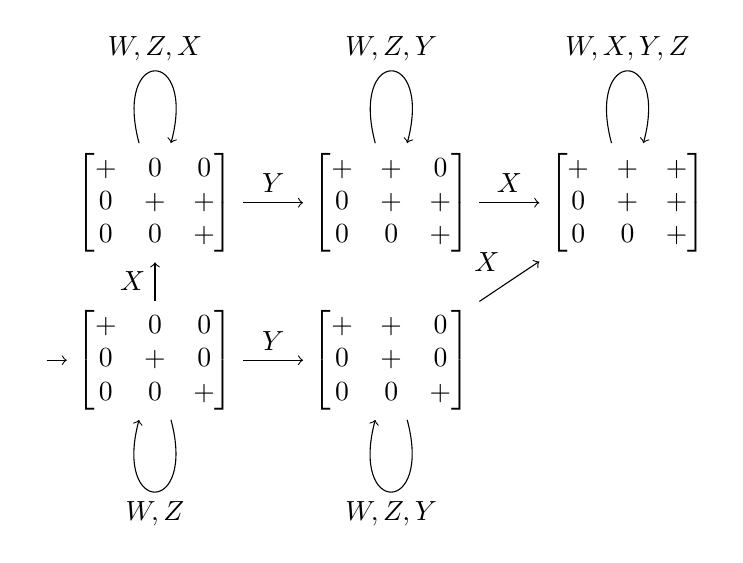
\begin{tikzpicture}
    \node(start) at (-1.5,0) {};
    \node(id) at (0,0) {$\begin{bmatrix}+&0&0\\0&+&0\\0&0&+\end{bmatrix}$};
    \node(cp) at (0,2) {$\begin{bmatrix}+&0&0\\0&+&+\\0&0&+\end{bmatrix}$};
    \node(acp) at (3,2) {$\begin{bmatrix}+&+&0\\0&+&+\\0&0&+\end{bmatrix}$};
    \node(ap) at (3,0) {$\begin{bmatrix}+&+&0\\0&+&0\\0&0&+\end{bmatrix}$};
    \node(abcp) at (6,2) {$\begin{bmatrix}+&+&+\\0&+&+\\0&0&+\end{bmatrix}$};
    \draw[->] (start) -- (id);
    \draw[->] (id) to node[auto] {$X$} (cp);
    \draw[->] (id) to node[auto] {$Y$} (ap);
    \draw[->] (cp) to node[auto] {$Y$} (acp);
    \draw[->] (acp) to node[auto] {$X$} (abcp);
    \draw[->] (ap) to node[auto] {$X$} (abcp);
    \draw[->,loop below] (id) to node[auto] {$W,Z$} (id);
    \draw[->,loop below] (ap) to node[auto] {$W,Z,Y$} (ap);
    \draw[->,loop above] (cp) to node[auto] {$W,Z,X$} (cp);
    \draw[->,loop above] (acp) to node[auto] {$W,Z,Y$} (acp);
    \draw[->,loop above] (abcp) to node[auto] {$W,X,Y,Z$} (abcp);
\end{tikzpicture}
\end{center}
Starting from the identity and applying the different products $e^{A_{i}t_{i}}$ in the automaton,
it is clear that the only way to reach a matrix of the shape of $G$ is to have all
the ``$X$'' before ``$Y$''. Formally, by contradiction, if there were $i<j$ such
that $A_{i}=Y$ and $A_{j}=X$ then by the automaton, we would end up with a matrix where
the top right corner is nonzero, which contradicts $G=\prod_{i=1}^{p} e^{A_{i} t_{i}}$.
\end{proof}

The previous lemma shows that this semigroup enforces a partial order on the matrices
in products that reach the matrix $G$. The next lemma shows that $G$ can indeed be reached using this
kind of products, essentially proving that $G$ belongs to this semigroup.

\begin{proposition}\label{prop:forced_order_exists}
For any positive real $t$, there exists a non-negative real $u$ such that
\[e^{Wu}e^{Xt}e^{Yt}e^{Zu}=G\quad\text{ or }\quad e^{Zu}e^{Xt}e^{Yt}e^{Wu}=G.\]
\end{proposition}

\begin{proof}
Consider the following products for an arbitrary $u\geqslant0$:
\begin{align*}
e^{Wu}e^{Xt}e^{Yt}e^{Zu}&=\begin{bmatrix}1&0&0\\0&e^u&0\\0&0&e^{2u}\end{bmatrix}
    \begin{bmatrix}1&t&0\\0&1&t\\0&0&1\end{bmatrix}
\begin{bmatrix}1&0&0\\0&e^{-u}&0\\0&0&e^{-2u}\end{bmatrix}\\[5pt]
&=\begin{bmatrix}1&0&0\\0&e^u&0\\0&0&e^{2u}\end{bmatrix}
\begin{bmatrix}1&te^{-u}&0\\0&e^{-u}&te^{-2u}\\0&0&e^{-2u}\end{bmatrix}\\[5pt]
&=\begin{bmatrix}1&te^{-u}&0\\0&1&te^{-u}\\0&0&1\end{bmatrix},
\end{align*}
and
\[
e^{Zu}e^{Xt}e^{Yt}e^{Wu}=\begin{bmatrix}1&te^{u}&0\\0&1&te^{u}\\0&0&1\end{bmatrix}.
\]
If $t\geqslant1$ then choosing $u=\ln t\geqslant0$ in the first product gives $G$,
otherwise choosing $u=\ln\frac{1}{t}\geqslant0$ in the second product gives $G$.
\end{proof}

\subsection{Undecidability of the Semigroup Membership Problem}

We will now show the undecidability of MSMP\@. 

In short, the difference is that we do not fix the order of the matrices in the product, and that each matrix may be used more than once. We will now show the following key result.

\begin{theorem}
  MSMP is undecidable in the non-commutative case.
\end{theorem}

\begin{proof}
We have seen in the previous section that MEP is undecidable in the non-commutative
case. Thus it suffices to reduce MEP to MSMP to show undecidability.

Let $A_1,\ldots,A_k,C\in\Algebraics^{n\times n}$ be an instance of MEP\@. Denote by $I_m$ the identity of size $m$,
$0_m$ the zero matrix of size $m$. Recall the $3 \times 3$ matrices $W,X,Y,Z,G$, defined in \cref{sec:lics_gadget}.
For every $i\in\lbrace 2,\ldots,k-1\rbrace$, define the following matrices:
\begin{align*}
&B_{i}=\begin{bmatrix}A_{i}&&&&\\&0_{3(i-2)}&&&\\&&Y&&\\&&&X&\\&&&&0_{3(k-1-i)}\end{bmatrix},
&B_{i}'=\begin{bmatrix}0_n&&&&\\&0_{3(i-2)}&&&\\&&Y&&\\&&&X&\\&&&&0_{3(k-1-i)}\end{bmatrix}.
\end{align*}

We also define the matrices
\begin{align*}
&B_1=\begin{bmatrix}A_1&&\\&X&\\&&0_{3(k-2)}\end{bmatrix},&&
&B_1'=\begin{bmatrix}0_n&&\\&X&\\&&0_{3(k-2)}\end{bmatrix},\\[5pt]
&B_k=\begin{bmatrix}A_1&&\\&0_{3(k-2)}&\\&&Y\end{bmatrix},&&
&B_k'=\begin{bmatrix}0_n&&\\&0_{3(k-2)}&\\&&Y\end{bmatrix},\\
\end{align*}
and, for every $i\in\lbrace 1,\ldots,k-1\rbrace$,
\begin{align*}
&W_{i}=\begin{bmatrix}0_n&&&\\&0_{3(i-1)}&&\\&&W&\\&&&0_{3(k-1-i)}\end{bmatrix},
&Z_{i}=\begin{bmatrix}0_n&&&\\&0_{3(i-1)}&&\\&&Z&\\&&&0_{3(k-1-i)}\end{bmatrix}.
\end{align*}

Finally, we define the target matrix:
\[C'=\begin{bmatrix}C&&&\\&G&&\\&&\ddots&\\&&&G\end{bmatrix}.\]
We can now define our MSMP instance as follows, the target matrix is $C'$ and the semigroup $\mathcal{G}$
is generated by
\begin{align*}
&\left\lbrace e^{B_{i}t_{i}},e^{B_{i}'t_{i}}:t_{i}\geqslant0,i=1,\ldots,k\right\rbrace \\
&\cup\left\lbrace e^{W_{i}t_{i}},e^{Z_{i}t_{i}}:t_{i}\geqslant0,i=1,\ldots,k-1\right\rbrace.
\end{align*}
We claim the original instance of MEP is satisfiable if and only if $C'\in\mathcal{G}$.
Let us examine both directions independently.

Assume that the MEP instance is satisfiable. Then there exist $t_1,\ldots,t_k\geqslant0$ such that:
\[\prod_{i=1}^{k}e^{A_{i}t_{i}}=C.\]
Define $\tau=\max\lbrace t_1,\ldots,t_k\rbrace+1$ (note that $\tau>0$) and $t_{i}'=\tau-t_{i}\geqslant0$ for every $i\in\lbrace 1,\ldots,k\rbrace$.
A straightforward calculation shows that:
\begin{align*}
\prod_{i=1}^{k}\left(e^{B_{i}t_{i}}e^{B_{i}'t_{i}'}\right)
    &=\begin{bmatrix}\prod_{i=1}^{k}e^{A_{i}t_{i}}&&&\\&e^{X\tau}e^{Y\tau}&&\\&&\ddots&\\&&&e^{X\tau}e^{Y\tau}\end{bmatrix}\\
    &=\begin{bmatrix}C&&&\\&U&&\\&&\ddots&\\&&&U\end{bmatrix},
\end{align*}
where $U=e^{X\tau}e^{Y\tau}$. Apply \cref{prop:forced_order_exists} to get $\lambda\geqslant0$
such that either $e^{W\lambda}Ue^{Z\lambda}=G$ or $e^{Z\lambda}Ue^{W\lambda}=G$. In the first case, conclude by
checking that
\[
\prod_{i=1}^{k-1}e^{W_{i}\lambda}\prod_{i=1}^{k}\left(e^{B_{i}t_{i}}e^{B_{i}'t_{i}'}\right)\prod_{i=1}^{k-1}e^{Z_{i}\lambda}
    =\begin{bmatrix}C&&&\\&G&&\\&&\ddots&\\&&&G\end{bmatrix}=C'.
\]
In the second case, exchange the $W_{i}$ and $Z_{i}$ to get same result. This concludes the proof that
the MSMP instance is satisfiable, since all the products belong to $\mathcal{G}$.

Assume that the MSMP instance is satisfiable. Then there exist $t_1,\ldots,t_m>0$ (we can always take them positive)
and $M_1,\ldots,M_m\in\big\lbrace B_{i},B_{i}':i=1,\ldots,k\rbrace\cup\big\lbrace W_{i},Z_{i}:i=1,\ldots,k-1\big\rbrace$
such that
\begin{equation}\label{eq:mesp_to_mep:prod_eq}
\prod_{j=1}^{m}e^{M_{j}t_{j}}=C'.
\end{equation}
Observe that by construction, this product has the following form:
\[\prod_{j=1}^{m}e^{M_{j}t_{j}}=\begin{bmatrix}V&&&\\&U_1&&\\&&\ddots&\\&&&U_{k-1}\end{bmatrix},\]
where $V$ belongs to the semigroup generated by $\lbrace e^{A_{i}t}:t\geqslant0\rbrace$ and $U_{i}$ belongs
to the semigroup generated by $\lbrace e^{Wt},e^{Xt},e^{Yt},e^{Zt}:t\geqslant0\rbrace$. Since
\eqref{eq:mesp_to_mep:prod_eq} implies that $U_{i}=G$, we can apply \cref{prop:eq_has_forced_order}
to get each product producing $U_{i}$ must have all its ``$X$'' before its ``$Y$''. Furthermore, each $U_{i}$
must contain at least one $X$ and one $Y$ in its product. For any $i\in\lbrace 1,\ldots,k\rbrace$,
let $k_{i}$ (resp., $k_{i}'$) denote
the first (resp., last) index $j$ such that $M_{j}=B_{i}\text{ or }B_{i}'$. Those indices exist because
of the proposition since at least one $B_{i}$ or $B_{i}$' must appear for every $i$
to get both an $X$ and a $Y$ in each product giving $U_{i}$. Obviously $k_{i}\leqslant k_{i}'$
by definition. We now claim that the proposition implies that:
\[k_1\leqslant k_1'<k_2\leqslant k_2'<k_3\cdots<k_{k-1}\leqslant k_{k-1}'.\]
Indeed, \cref{prop:eq_has_forced_order} ensures that in the product giving $U_1$,
all the ``$X$'' appear before the ``$Y$'',
but the only matrices that contribute some $X$ to $U_1$ are $B_1$ and $B_1'$,
and the only matrices that contribute some $Y$ to $U_1$ are $B_2$ and $B_2'$.
Thus $k_1'<k_2$, i.e. the last ``$X$'' coming from $B_1$ or $B_1'$ is before the first ``$Y$''
coming from $B_2$ or $B_2'$. A similar reasoning ensures that $k_2'<k_3$ and so on.
This shows that for any $i\in\lbrace 1,\ldots,k\rbrace$, if $M_{j}=B_{i}$ then $j\in\lbrace k_{i},\ldots,k_{i}'\rbrace$. Thus all
the $B_1$ appear before the $B_2$ which appear before the $B_3$ and so on.
However, since the $B_{i}$ are the only ones to contribute to $V$, then $V$ must be of the form:
\[V=\prod_{i=1}^{k}e^{A_{i}t_{i}'},\]
where $t_{i}'\geqslant0$ is the sum of all $t_{j}$ such that $M_{j}=B_{i}$.
Finally $V=C$, so the instance of MEP is satisfiable.

\end{proof}

\section{Vector and Hyperplane Reachability}

In this section we show that the vector and halfspace reachabililty
problems for matrix-exponential semigroups, as given in
\cref{def:generalised-problems}, are both undecidable.

\begin{theorem}
The Matrix-Exponential Vector Reachability Problem is undecidable.
\end{theorem}

\begin{proof}
This can be shown by reduction from the membership problem for
matrix-exponential semigroups. In particular, given square matrices
$B_{1}, \ldots, B_{k}, C$, we construct matrices $A_{1}, \ldots,
A_{k}$ and vectors $\myvector{x}, \myvector{y}$ for which
\begin{equation}
  \label{eq:mesp-to-orbit}
  \prod \limits_{j=1}^{m} \exp(B_{i_{j}} t_{j}) = C \Leftrightarrow
  \prod \limits_{j=1}^{m} \exp(A_{i_{j}} t_{j}) \myvector{x} = \myvector{y} .
\end{equation}

Let $\myvector{c}_{1}, \ldots, \myvector{c}_{n}$ be the columns of
$C$, from left to right, and let $\myvector{e}_{1}, \ldots,
\myvector{e}_{n}$ denote the canonical basis of
$\Reals^{n}$. Then~\eqref{eq:mesp-to-orbit} can be achieved by
setting, for each $i \in \lbrace 1, \ldots, n \rbrace$,
\begin{equation*}
A_{i} =
\begin{pmatrix}
B_{i} && \cdots && 0 \\
\vdots && \ddots && \vdots \\
0 && \cdots && B_{i}
\end{pmatrix} \in \Reals^{n^{2} \times n^{2}},
\end{equation*}
as well as
\begin{equation*}
\myvector{x} = \begin{pmatrix} \myvector{e}_{1} \\ \vdots \\ \myvector{e}_{n} \end{pmatrix} \mbox{ and }
\myvector{y} = \begin{pmatrix} \myvector{c}_{1} \\ \vdots \\ \myvector{c}_{n} \end{pmatrix} \, .
\end{equation*}
\end{proof}

\begin{theorem}
The Matrix-Exponential Hyperplane Reachability Problem is undecidable.
\end{theorem}

\begin{proof}
This can be shown by reduction from the vector reachability problem.
Similarly to what we did in the previous proof, we will define
matrices $C_{1}, \ldots, C_{k}$ and vectors $\myvector{w},
\myvector{z}$ such that
\begin{equation*}
\prod \limits_{i=1}^{k} \exp(A_{i} t_{i}) \myvector{x} = \myvector{y}
\Leftrightarrow
\myvector{w}^{T} \prod\limits_{i=1}^{k} \exp(C_{i} t_{i}) \myvector{z} = 0 \, .
\end{equation*}

Let $\myvector{e}_{1}, \ldots, \myvector{e}_{n}$ denote the canonical basis of $\Reals^{n}$. Moreover, let
\begin{equation*}
B_{i} = \begin{pmatrix} A_{i} && 0 \\ 0 && 0 \end{pmatrix},
\myvector{u}_{j} = \begin{pmatrix} \myvector{e}_{j} \\ - \myvector{e}_{j} \end{pmatrix},
\myvector{v} = \begin{pmatrix} \myvector{x} \\ \myvector{y} \end{pmatrix}
\end{equation*}
and
\begin{equation*}
C_{i} = \begin{pmatrix} B_{i} \otimes I + I \otimes B_{i} && \cdots && 0 \\ \vdots && \ddots && \vdots \\ 0 && \cdots && B_{i} \otimes I + I \otimes B_{i} \end{pmatrix} \, .
\end{equation*}
Then
\begin{align*}
&\prod \limits_{i=1}^{k} \exp(A_{i} t_{i}) \myvector{x} = \myvector{y} \\
\Leftrightarrow &\sum \limits_{j=1}^{n} \left( \myvector{u}_{j}^{T} \prod \limits_{i=1}^{k} \exp(B_{i} t_{i}) \myvector{v} \right)^{2} = 0 \\
\Leftrightarrow &\sum \limits_{j=1}^{n} \left( \left( \myvector{u}_{j} \otimes \myvector{u}_{j} \right)^{T} \prod \limits_{i=1}^{k} \left( \exp( B_{i} t_{i} ) \otimes \exp(B_{i} t_{i}) \right) \left( \myvector{v} \otimes \myvector{v} \right) \right) = 0 \\
\Leftrightarrow &\sum \limits_{j=1}^{n} \left( \left( \myvector{u}_{j} \otimes \myvector{u}_{j} \right)^{T} \prod \limits_{i=1}^{k} \exp\left((B_{i} \otimes I + I \otimes B_{i}) t_{i} \right) \left( \myvector{v} \otimes \myvector{v} \right) \right) = 0 \\
\Leftrightarrow &\begin{pmatrix} \myvector{u}_{1} \otimes \myvector{u}_{1} \\ \vdots \\ \myvector{u}_{n} \otimes \myvector{u}_{n} \end{pmatrix}^{T} \prod \limits_{i=1}^{k} \exp( C_{i} t_{i} ) \begin{pmatrix} \myvector{v} \otimes \myvector{v} \\ \vdots \\ \myvector{v} \otimes \myvector{v} \end{pmatrix} = 0 .
\end{align*}

The result then follows by taking
\begin{equation*}
  \myvector{w} = \begin{pmatrix} \myvector{u}_{1} \otimes \myvector{u}_{1} \\ \vdots \\ \myvector{u}_{n} \otimes \myvector{u}_{n} \end{pmatrix}
  \mbox{ and } \myvector{z} = \begin{pmatrix} \myvector{v} \otimes \myvector{v} \\ \vdots \\ \myvector{v} \otimes \myvector{v} \end{pmatrix} \, .
\end{equation*}
\end{proof}

\section{Turing-degree of MSMP}
\label{sec:turing-degree-lics}

We are interested in classifying the Turing-degree of MSMP\@.  Recall
that the first level of the arithmetical hierarchy, denoted
$\Sigma_1$, consists of the recursively enumerable languages, while
the second level of the arithmetical hierarchy, denoted $\Sigma_2$,
consists of the languages that can be enumerated by a Turing machine
with an oracle to a language in $\Sigma_1$.


\begin{theorem}
\label{thm:turing-degree-2}
$\mbox{MSMP}$ lies in $\Sigma_2$.
\end{theorem}

\begin{proof}
Given an instance of MSMP, determined by generating matrices $A_1,\ldots,A_k$ and target $C$,
consider the functions $f_{\myvector{w}} : \mathbb{R}^{|\myvector{w}|} \rightarrow \Reals$,
defined for each $\myvector{w} \in {\lbrace 1, \ldots, k \rbrace}^*$ by
\begin{equation*}
    f_{\myvector{w}}(\myvector{t}) = {\left \| \prod \limits_{i=1}^{\lvert \myvector{w} \rvert} \exp(A_{w_{i}} t_{i}) - C \right \|}_{F}^2 \, ,
\end{equation*}
where $\| \cdot \|_F$ denotes the Frobenius norm of a matrix (obtained
as the positive square root of the sum of the squares of the matrix entries).  Note that each
$f_{\myvector{w}}$ is an exponential-polynomial which takes values in
the nonnegative reals. Clearly, the given instance of MSMP is positive
if and only if some $f_{\myvector{w}}$ has a (necessarily tangential)
zero.

Before proceeding, note that exponential-polynomials are closed under differentiation, and that they are computable functions.

Let $\myvector{b} : \Naturals \rightarrow {\lbrace 1, \ldots, k
  \rbrace}^*$ be any computable surjection.
For each $n \in \Naturals$ and $\myvector{w} \in \lbrace
\myvector{b}(1), \ldots, \myvector{b}(n) \rbrace$, consider the Turing
machine $A_{\myvector{w}, n}$ that does the following: for each $m
\in \Naturals$, partition ${[0,n]}^{\lvert \myvector{w} \rvert}$ in a
uniform grid, with mesh size $m^{-1}$, and compute the approximate
value of $f_{\myvector{w}}$ with error at most $m^{-1}$ at each grid
point; if it is ever the case that all the approximate values of
$f_{\myvector{w}}$ are greater than $\left(1+ \frac{L_{\myvector{w},
    n}\sqrt{\lvert \myvector{w} \rvert}}{2} \right) m^{-1}$ (where
$L_{\myvector{w}, n}$ is an upper bound on ${\| \nabla
  f_{\myvector{w}} \|}\restriction_{[0,n]}$, which we can compute by
using the triangle inequality and the monotonicity of the exponential
function), $A_{\myvector{w}, n}$ halts.  Due to the Mean Value Theorem
and to the compactness of $[0,n]$, $A_{\myvector{w}, n}$ halts if and
only if $f_{\myvector{w}} \restriction_{[0,n]}$ does not have a zero.
Thus, the instance of MSMP is positive if and only if some
$A_{\myvector{w}, n}$ does not halt.

Now, consider the Turing machine $B$ with access to an oracle for the  Halting Problem
that, for each $n \in
\Naturals$ and $\myvector{w} \in \lbrace \myvector{b}(1), \ldots,
\myvector{b}(n) \rbrace$, uses the oracle to decide whether
$A_{\myvector{w}, n}$ halts and $B$ only if halts if some oracle 
call determines that $A_{\myvector{w}, n}$ runs forever.
Then $B$ halts if and only if the MSMP instance
in consideration is positive.
\end{proof}

Moreover, the following result holds.

\begin{theorem}
\label{thm:turing-degree-1}
If Schanuel's conjecture is true then $\mbox{MSMP}$ lies in $\Sigma_1$.
\end{theorem}

\begin{proof}
Let $f_{\myvector{w}}, \myvector{w} \in {\lbrace 1, \ldots, k
  \rbrace}^{\star}$ be as in the proof of~\cref{thm:turing-degree-2}.
Consider the Turing Machine $T$ which, for each $n \in \Naturals$ and
$\myvector{w} \in \lbrace \myvector{b}(1), \ldots, \myvector{b}(n)
\rbrace$, uses~\cref{thm:wilkie-macintyre} to decide whether
$f_{\myvector{w}}$ admits a zero in the region ${[0,n]}^{\lvert
  \myvector{w} \rvert}$, and halts when such a zero is found.  Then
$T$ halts if and only if the instance of MSMP under consideration is
positive.
\end{proof}

\section{Conclusion}

We have shown that the Matrix-Exponential Semigroup Membership Problem
is undecidable in general, but decidable when the generating matrices
$A_{1}, \ldots, A_{k}$ commute.  Our results are analogous to what is
known for the discrete version of this problem--the Matrix Semigroup
Membership Problem--namely decidability in the commutative case and
undecidability in general (see Section~\ref{sec:lics_related_work}).
Finally, we have shown that the Matrix-Exponential Semigroup
Membership Problem is in $\Sigma_{1}$ if Schanuel's conjecture is
true, and in $\Sigma_{2}$ unconditionally. Note that for the Matrix
Semigroup Membership Problem, membership in $\Sigma_{1}$ follows
trivially from the fact that a finitely generated matrix semigroup is
recursively enumerable.

It would be interesting to look at possibly decidable restrictions of
Matrix-Exponential Semigroup Membership Problem: for example, the case
with two non-commuting generators, which was shown to be decidable in
the case of the analogous discrete problem in~\cite{MEHTP}. Bounding
the dimension of the ambient vector space might also yield
decidability, along the lines of results in the discrete case
in~\cite{PS2Z}.  Finally, deriving upper and lower bounds for the
computational complexity of the commutative case remains to be
addressed.

\bibliography{refs}
\bibliographystyle{plain}

\end{document}

